%% thesis.tex 2014/04/11
%
% Based on sample files of unknown authorship.
%
% The Current Maintainer of this work is Paul Vojta.

\documentclass[titlepage]{ucbthesis}
\usepackage{rotating} % provides sidewaystable and sidewaysfigure
\usepackage[utf8]{inputenc}
%\usepackage[english]{babel}
\usepackage[backend=biber,style=chem-acs,sorting=none]{biblatex} % Bibliography
\addbibresource{referencias.bib}
\setcounter{tocdepth}{1} % Depth for TOC numeration
\setcounter{secnumdepth}{1}
\usepackage{amsmath}
\usepackage{bm}
\usepackage{amssymb}
\usepackage{graphicx}
\usepackage{wrapfig}
\usepackage{subcaption}
\usepackage{dcolumn}
%\usepackage{capt-of}
\usepackage[labelfont=bf,labelsep=period]{caption}
\graphicspath{ {.\images} }
\usepackage{cancel}
\usepackage[most]{tcolorbox}
\usepackage{afterpage}
\usepackage{multirow}
\usepackage[flushleft]{threeparttable}
\usepackage{ragged2e}
\usepackage[]{fancyhdr}
\fancypagestyle{resumenheader}
{
    \fancyhead[C]{Simulation of rolling magnetic microswarms along acoustic virtual walls by coupling a Lattice-Boltzmann scheme and molecular dynamics}    
}
% To compile this file, run "latex thesis", then "biber thesis"
% (or "bibtex thesis", if the output from latex asks for that instead),
% and then "latex thesis" (without the quotes in each case).

% Double spacing, if you want it.  Do not use for the final copy.
% \def\dsp{\def\baselinestretch{2.0}\large\normalsize}
% \dsp

% If the Grad. Division insists that the first paragraph of a section
% be indented (like the others), then include this line:
\usepackage{indentfirst}

\addtolength{\abovecaptionskip}{\baselineskip}

\newtheorem{theorem}{Jibberish}

\hyphenation{mar-gin-al-ia}
\hyphenation{bra-va-do}

\begin{document}
\renewcommand{\figurename}{Fig.}
\renewcommand{\tablename}{Chart}
\renewcommand{\listtablename}{chart index}
\setlength{\abovecaptionskip}{10pt}
\setlength{\belowcaptionskip}{10pt}
% Declarations for Front Matter

\title{Simulation of rolling magnetic microswarms along acoustic virtual walls by coupling a Lattice-Boltzmann scheme and molecular dynamics}
%\title{Simulación de rotores magnéticos moviéndose en paredes virtuales acústicas acoplando un método de Lattice-Boltzmann y dinámica molecular}
\author{Esteban Castro Ávila}
\degreeyear{2023}
%\degree{Magíster}
\degree{Master in science -}
% For a co-chair who is subordinate to the \chair listed above
% \cochair{Professor Benedict Francis Pope}
% For two co-chairs of equal standing (do not use \chair with this one)
% \cochairs{Professor Richard Francis Sony}{Professor Benedict Francis Pope}
% Previous degrees are no longer to be listed on the title page.
% \prevdegrees{B.A. (University of Northern South Dakota at Hoople) 1978 \\
%   M.S. (Ed's School of Quantum Mechanics and Muffler Repair) 1989}
\field{Physics}
%\field{Ciencias, Química}
% Designated Emphasis -- this is optional, and rare
% \emphasis{Colloidal Telemetry}
% This is optional, and rare
% \jointinstitution{University of Western Maryland}
% This is optional (default is Berkeley)
% \campus{Berkeley}

% For a masters thesis, replace the above \documentclass line with%
%\documentclass[masters]{ucbthesis}
% This affects the title and approval pages, which by default calls this
% document a "dissertation", not a "thesis"%

\maketitle
\makesubtitle

% Delete (or comment out) the \approvalpage line for the final version.
%\approvalpage
%\copyrightpage

\begin{frontmatter}

\begin{dedication}
\begin{flushright}
\begin{vplace}
\textit{To my family.}
\vspace{3cm}
\textit{``The imagination of nature is far,\\
far greater than the imagination of man."}
\vspace{0.1cm}
\textit{-Richard P. Feynman}
\end{vplace}
\end{flushright}
\end{dedication}

% You can delete the \clearpage lines if you don't want these to start on
% separate pages.

\addcontentsline{toc}{chapter}{Acknowledgements}

\chapter*{Acknowledgements}

In the first place I wish to express my gratefulness to the National University of Colombia for letting me to be formed as scientist and supporting me with opportunities as the Academic rights Exception and the Auxiliary Professor scholarships. In the second place, to thank the Helmholtz Institute of Erlangen-Nürmberg for renewable energy (HI-ERN), especially to the professor Dr. Jens Harting, for inviting me as guest scientist to collaborate in the development of the software LB3D and to Jülich Forschungzentrum for financing the flight tickets needed to complete a four months research stay at Erlangen, Germany. In the same manner I would  like to thank the University center of Bayern for Latin-America (BAYLAT) for supporting me financially during the research stay in Erlangen through a scholarship. Also, I would like to give of course gratefulness to my family who was supporting me emotionally during these recent years to learn new things and grow professionally, as well to the Thesis advisor Dr. Ret-Nat Jos\'{e} Daniel Mu\~{n}oz for the numerous lessons taught to me in the academics and professional life, to my co-advisor Dr. Paolo Malgaretti for his essential contribution on this project and providing knowledge about academic research strategies. In the same manner I wish to thank to all colleagues and partners at HI-ERN who guided me through the completion of this project such as Dr. Othmane Aouane and Johannes Hielscher, among others, and finally to all colleagues from the National University for the given emotional support during this post-graduate program. \\

%En primer lugar deseo expresar mi agradecimiento con la Universidad Nacional de Colombia por permitirme formarme como hombre de ciencia y por su colaboración económica y laboral mediante las becas de Exención de Derechos Académicos y Auxiliar Docente. En segundo lugar agradecer al \textit{Helmholtz Institute Erlangen-Nürmberg for renewable energy} (HI-ERN), por recibirme como invitado a colaborar en el desarrollo del software LB3D y haber financiado los viajes de ida y vuelta a la ciudad de Erlangen, ubicada en Alemania, para realizar una estadía de investigación de cuatro meses enfocada al desarrollo de este proyecto. Del mismo modo agradezco al Centro Universitario de Baviera para América Latina (BAYLAT) por financiar mi manutención durante la estadía de investigación en Erlangen. Quiero por supuesto agradecerle a mi familia, quienes han sido fuente de apoyo incondicional durante todos estos años y me han motivado a aprender más y más. Al profesor Dr. Ret-Nat José Daniel Muñoz de mi grupo de investigación por las numerosas lecciones sobre los temas que me apasionan y por su apoyo sincero en temas fuera de lo académico, al profesor Dr. Paolo Malgaretti por su esencial apoyo como co-director en este proyecto y por brindar importantes conocimientos en el ámbito investigativo y académico. De la misma forma a mis colegas, tanto a los presentes como a aquellos que han partido a cumplir sus sueños muy lejos de nuestro hogar, por formar parte de mi formación mediante críticas constructivas y debates académicos. Y, por supuesto, a mis directores de trabajo de grado quienes me han guiado durante todo este proceso de formación como investigador. Agradezco enormemente las oportunidades que ellos me han brindado, entre ellas cursar esta primer etapa de estudios de posgrado.

\addcontentsline{toc}{chapter}{Abstract}
\thispagestyle{resumenheader}

\chapter*{Resumen}

.\\

\hspace{-0.6cm}\textbf{Palabras clave: }.

\clearpage

\chapter*{Abstract}

.\\

\hspace{-0.6cm}\textbf{Keywords: }.

\tableofcontents
\clearpage
\listoffigures
\clearpage
\listoftables

\end{frontmatter}

\pagestyle{headings}

%%%%%%%%%  Cuerpo del documento  %%%%%%%%%
\part{Introduction}
\chapter{Introduction}
%JUSTIFICACION
\begin{figure}[b]
    \centering
    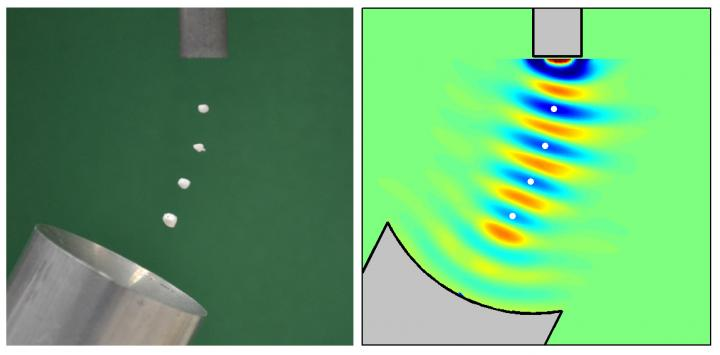
\includegraphics[width=0.45\textwidth]{images/intro/ac_levitaion_1.jpg}
    \caption{Example of acoustic levitation using acoustical tweezers.}
    \label{fig:ac_lev}
\end{figure}
The study of the motion of microswimmers in aqueous media has won relevance in the recent years, because of its applications in biotechnology, biodiversity, health research, marine research and earth science, among others. Microswarms are microscopical bodies usually transported using external acoustic, magnetic or electrostatic fields to transport self-assembled structures without contact \cite{Mohanty2020,Harting2021,Shi2009}.

One way of controlling the motion of microparticles in a fluidic medium is by using acoustical tweezers, which are built from a pressure sound transducer opposing a reflecting surface (see figure \ref{fig:ac_lev}) or an array of phase-modulated transducers capable of generating standing acoustic waves such that pressure nodes are focused on the object to be moved as seen in figure \ref{fig:ac_tw_surgery} where standing waves hold a small object \cite{Shi2009, Marzo2015}. As the preceding optical tweezers generate standing electromagnetic waves to manipulate microscopical objects like viruses, cells or bacteria, acoustic waves can manipulate particles, cells or micro-bodies of any shape, charge or polarity, as soon as it size is much smaller than the wavelength of the standing acoustic wave. Nevertheless, acoustic tweezers requires 5$\times$10$^5$ times less power than optical tweezers. Indeed, they can move objects from 100 nm to 10 mm large with intensities from $10^{-2}$ to 10 W/cm$^2$ for the input source, unlike optical tweezers, which requires more than $10^{6}$ W/cm$^2$ \cite{Ozcelik2018}. 

One common application for acoustical tweezers are non-invasive surgeries, preventing bleeding, infection, scarring or anesthesia complications caused by incisions, punctures and instrument insertions in invasive surgery, which occur in one out of six patients. Also, external magnetic, electrostatic, acoustic fields can be also used to control the clustering of particles and create self-assembled structures, leading the development of microbots \cite{Ghanem2020, Kaiser2017}. 
\begin{figure}[t]
    \begin{subfigure}{.38\columnwidth}
    \centering
    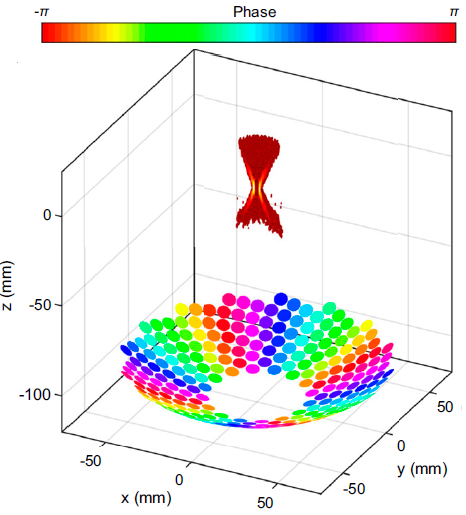
\includegraphics[width=\textwidth]{images/intro/surgery_acTweezer.PNG}
    \caption{}
    \label{fig:ac_tw_surgery}
    \end{subfigure}
    \begin{subfigure}{.58\columnwidth}
    \centering
    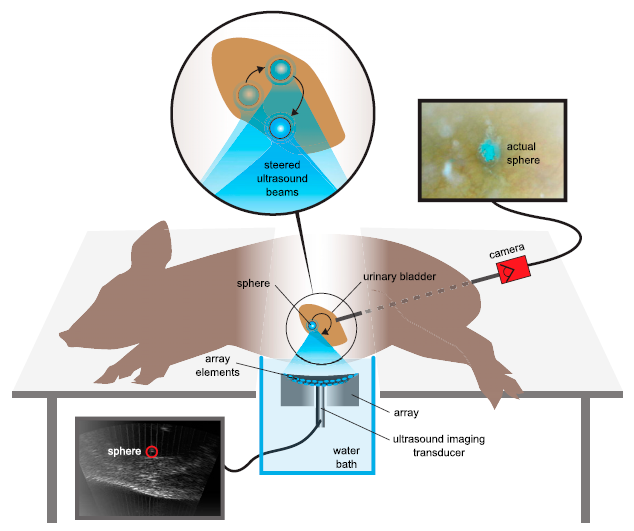
\includegraphics[width=\textwidth]{images/intro/surgery.PNG}
    \caption{}
    \label{fig:pig_surgery}
    \end{subfigure}
    \caption{Focal acoustic tweezer made of an array of transducers to develop surgeries (a), surgery for the extraction of a urinary stone of a pig.}
    \label{fig:pig}
\end{figure}
\section{Previous works}
%ESTADO DEL ARTE

The manipulation of small objects with fields began with the 2018 Nobel Prize study on optical tweezers, developed by Ashkin in 1970, which showed the possibility of trapping and accelerating dielectric particles using the stable potential well of a continuous laser. This result led to the birth of optical tweezers \cite{Ashkin1970}. Parallel to this research, in 1962 the Russian physicist Lev Petrovich Gor'kov, based on King's works on acoustical radiation forces \cite{King1934, King1935}, studied the force exerted by an acoustical field on a spherical particle immersed in an ideal fluid and deduced the so-called Gor'kov potential, which is the basic principle of acoustical tweezers \cite{Gorkov1962}. 
%In Gor'kov's work the force is obtained as the gradient of a multipolar expansion of the velocity potential. 
Further theoretical improvements of the model were done by J. Wu and G. Du in 1990, even proving their results with experiments where  latex particles were confined using two focused PZT transducers \cite{WuDu1990,Wu1991}. Later experiments were carried out to create acoustical traps lab chips to move an array of colloidal particles in the three orthogonal directions of space \cite{Shi2009}. 

%AQUI VOY jdmunozc

Other developments were made of transducer arrays to larger applications like the non-invasive kidney stone expulsion of a pig as seen in figure \ref{fig:pig}. The surgery consisted in manipulating urinary stones to be extracted without making incisions. The surgery was accomplished without damages in the organ tissue, demonstrating the potential of acoustical tweezers for medicine applications \cite{Ghanem2020}. With this potential, micro-robotics has been studied in this field, whether for surgery or drug delivery, as it was proposed by Feynman as "swallowing the surgeon". Self-assembling of micro-beads is the path to develop micro-bots and it's inspired in nature swarms of many biological organisms \cite{Medina2017}. One way to produce clustering or self-assembling uses external rotating magnetic fields, where super-paramagnetic particles are aligned by its magnetic moment forming chains, vortex or ribbons depending on the orientation of controllable external fields. As it is seen from biological organisms like bacteria, spermatozoa, volvox among others particular ways to move and displace through aqueous fluids were viscous forces are dominating (very low Reynolds number), interaction of micro-particles with external fields have become an alternative to produce this kind of "swimming" motion. Many swimming mechanisms are studied from Scallop theorem, however rolling has been considered another motion alternative for micro-bots \cite{Purcell1977,Lauga2010}. The rolling motion has been also observed in nature, as the case of Neutrophil, and its displacement is due to friction with a surface or physical boundary. As micro-beads aggregate into disks or rods to develop rolling and additionally there is a strong dependence on gravity, which is not enough to keep a particle stuck to a wall. Acoustical waves have been used to keep a rolling motion in a surface in order to mimics the rolling motion of Neutrophil. The aggregation of particles to create wheel-like structures has been also carried out to study the dynamics of rolling through a vessel wall to create propulsion using a no-slip boundary condition \cite{Kaiser2017, Xie2019, Han2020,Harting2021,Tasci2015}. 

\begin{figure}[b]
    \begin{subfigure}{.38\columnwidth}
    \centering
    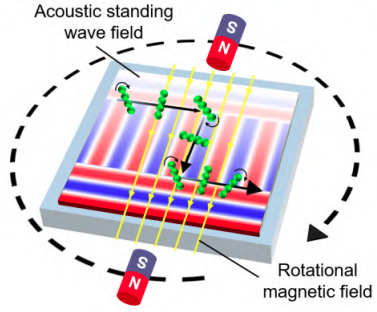
\includegraphics[width=\textwidth]{images/intro/microswimmers_generalScheme.png}
    \caption{}
    \label{fig:ms_gen}
    \end{subfigure}
    \begin{subfigure}{.38\columnwidth}
    \centering
    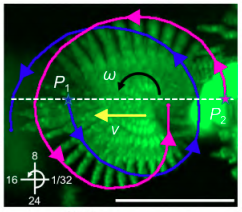
\includegraphics[width=\textwidth]{images/intro/microswimmers_rotation.png}
    \caption{}
    \label{fig:ms_rot}
    \end{subfigure}
    \begin{subfigure}{.8\columnwidth}
    \centering
    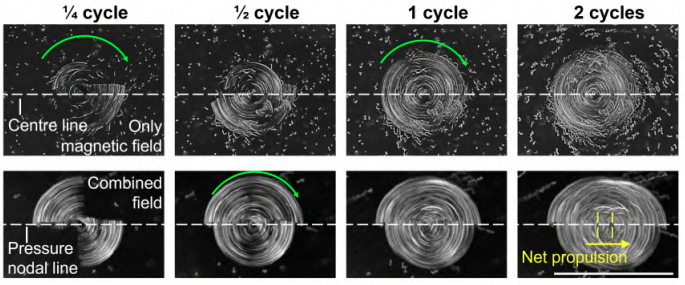
\includegraphics[width=\textwidth]{images/intro/microswimmers_cycles.png}
    \caption{}
    \label{fig:ms_cycles}
    \end{subfigure}
    \caption{General sketch of the rolling Microswimmers experiment (a). Graphical definition of the angular and linear speed of the Microswimmers (b) and comparison of the motion with and without standing waves (c).}
    \label{fig:LBMWaves}
\end{figure}

The rolling motion for chain-shaped microswarms has been studied experimentally by Harting, Malgaretti et. al. to be produced in virtual walls made by standing acoustic waves propagated through the medium \cite{paper_rods}. It is shown that this virtual boundary may be an alternative to develop rolling motion and the spatially asymmetrical hydrodynamic interactions and the help of an external, uniform and rotational magnetic field. The medium is surrounded by piezoelectric transducer which produces the acoustic standing waves along the medium and an acoustic radiation force is made by the particles to be enclosed, assembled into microchains and moving along the nodal plane (see figure \ref{fig:ms_gen}). This may be somehow analogous to the famous experiment of the Chladni patterns, where sand over a vibrating solid plate is being pushed to the nodal planes generated by vibration of the plate. However, this is an experiment taken into the microscopical scale where lengths are in the order of micrometers, the medium is an immerse fluid and instead of ordinary beads, there are microswarms which responds to magnetic fields and can be grouped into clusters instead of being assembled artificially. 
\begin{figure}[t]
    \centering
    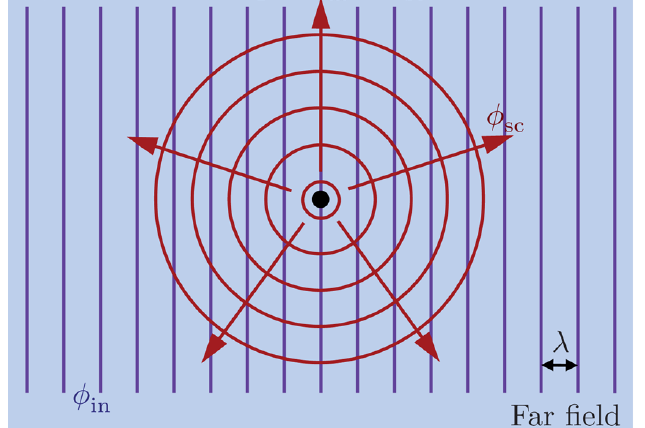
\includegraphics[width=0.45\textwidth]{images/intro/Scattering.PNG}
    \caption{Graphical representation of acoustical scattering where the velocity potential is decomposed into an incident and scattered field.}
    \label{fig:sc_scheme}
\end{figure}
Another key difference is that the acoustic fields may be plane waves guided by the walls in the boundaries instead of being normal modes whose pattern depends on the geometry of the medium and changes drastically with the driven frequency, which makes hard to control the form of the nodal planes. It was shown that the guiding of the nodal planes and the rotating magnetic field make possible the controlling of the motion of the microswarms, as there are linear relationships between the angular frequency of the rotating magnetic field and the linear speed of the microswarms, as well of a proportional relation between the wave's amplitude and the linear speed, shown in fig. \ref{fig:ms_rot}. It was also proved that the influence of the magnetic field by itself does not create a net displacement over the microswarms, therefor, the incident acoustic waves act like virtual boundaries which are useful to guide the movement of the particles as seen in the figure \ref{fig:ms_cycles}. 
\chapter{The theory behind the acoustic radiation force}

\section{Fluid dynamics concepts}\label{intro.sec:fluids}
In order to study the motion of fluids and elastic materials, it is necessary to describe this kind of physical system as a continuous medium where macroscopic variable are attributed, such as volume, density, pressure or other scalar or vector fields that may evolve in time and space (\cite{Landau} and \cite{Bruus2011_01}). The key reason behind the continuum hypothesis relies on the length scale of the total system to study. On lab-on-a-chip applications, where characteristic length scales are in the order of 100 $\mu$m similar to the magnetic microrotors experiment, there are already more than $10^{23}$ molecules per each space element of this size, thus, the system will be considered macroscopic. A limit for the length scale would be around 0.3 nm for fluids and 3 nm for gases, as these are characteristic order of magnitudes for inter-molecular distances, however, a minimum length to be dealt is not smaller than 10 $\mu$m, giving the possibility to develop all theoretical basis from continuum fluid mechanics \cite[sec.~1.1.2]{Bruus_book}. To be able to distinguish from one length scale to another, one the Knudsen number $\epsilon$ is used
\begin{equation}
    \epsilon = \frac{l_{\text{mfp}}}{L}
\end{equation}
the mean free path of the particles $l_{\text{mfp}}$ and the characteristic size of the system $L$. As this number is much less than unity, the continuum hypothesis is a valid treatment for fluids \cite[sec.~1.1]{Kruger}. In the continuum hypothesis any infinitesimal volume element is small compared to system size but large compared to the mean free path of particles, thus, there is no necessity on determining the dynamics of particles composed by the fluid but the dynamics of macroscopic fields dependent on the continuous space which are able to evolve in time. The description of these fields will be studied at any fixed position $\vec r = (x, y, z)$ of coordinates $r_1 = x$, $r_2 = y$ and $r_3 = z$ in the three-dimensional euclidean space. As Cartesian coordinates are used and tensorial fields are considered, the index notation is convenient to describe them. With index notation any vector $\vec A$ can be written as $A_i$ with $i=\{x_1,x_2,x_3\}\equiv\{x,y,z\}$, any matrix shall be written as $\mathbb{M} = M_{ij}$ and some symbols will be defined such as the Kronecker Delta $\delta_{ij}$ as a way to denote an identity matrix, and the Levi-Civita symbol $\epsilon_{ijk}$ valued 1 for any even permutation of $ijk$, -1 for any odd permutation of $ijk$ and 0 for any other case. An infinitesimal volume element of the fluid is taken such that will eventually move through all space. During an instant $\Delta t$ the fluid element makes a displacement that may be described by the vector displacement $D_i(\vec r,t)$. Also, at an instant $t$ the element will have an instantaneous velocity vector $u_i(\vec r,t)$ defined as
\begin{equation}\label{intro.fluids.eq:u_fluid_def}
    u_i = \frac{\partial D_i}{\partial t}\quad,
\end{equation}
This velocity is tracked only at $r_i$ instead of following the velocity of a same volume element which has moved after some time $\Delta t$ has passed. This way of describing the evolution of velocity or other fields is called an \textit{Eulerian picture} \cite{Bruus2011_01} which is the usual frame to describe the dynamic behavior of a fluid. 

Other relevant macroscopic fields to describe the fluid are the density $\rho(\vec r,t)$ of the volume element, which depend on the mass of each particle $m_i$ composed by the fluid element and its volume $\Delta V$, so that is defined as
\begin{equation}\label{intro.fluids.eq:rho_def}
    \rho(\vec r, t) = \frac{\sum_{n\in \Delta V}m_n}{\Delta V}\quad;
\end{equation}
the momentum $J_i(\vec r,t)$ per unit volume which is naturally defined as
\begin{equation}\label{intro.fluids.eq:J_def}
    J_i(\vec r, t) = \rho(\vec r, t)u_i(\vec r,t)\quad,
\end{equation}
and of course the following thermodynamics variables can be associated to the fluid as the pressure $P(\vec r,t)$ or temperature $T(\vec r,t)$, among others. 

These macroscopic fields are evolved in time and space by some partial differential equations which are defined as the following conservation laws: The mass conservation law and the momentum conservation law. Although energy conservation must also be included, this law shall be described instead using a thermodynamic state equation. Here will be presented the differential forms of these equations, if the reader is interested in the corresponding derivations, those are found in \cite{Landau} and \cite{Bruus_book}. The mass conservation is described with the continuity equation of the form
\begin{equation}\label{intro.fluids.eq:mass_conservation}
    \partial_t\rho + \partial_k(\rho u_k) = 0\quad,
\end{equation} 
where $\partial_t\equiv\partial/\partial t$ and  $\partial_i\equiv\partial/\partial x_i$. And the momentum conservation law is written as this vector partial differential equation:
\begin{equation}\label{intro.fluids.eq:momentum_conservation_law}
    \rho\partial_t u_i + \rho( u_k\partial_k)u_i = -\partial_i P + \eta\partial_k\partial_k u_i + \beta\eta\partial_i(\partial_k u_k)\quad,
\end{equation}
with $\eta$ the shear viscosity and $\beta$ a non-dimensional ratio. These last constants will be neglected as one of the limiting cases of this work, leading to a special form of the momentum equation called the \textit{Euler equation}:
\begin{equation}\label{intro.fluids.eq:euler_equation}
    \rho\partial_t u_i + \rho( u_k\partial_k)u_i = -\partial_i P \quad. 
\end{equation}
The force exerted by a fluid to an object immersed in the fluid is determined by the second law of Newton. This law basically states that any force made by the object is a momentum exchange between the fluid and the object. If the force per unit volume acting on the object is $F_i$ then the momentum change would be
\begin{equation}\label{intro.fluids.eq:force_fluid_def}
    f_i = \partial_t J_i\quad,
\end{equation}
then using \ref{intro.fluids.eq:J_def} and expanding the product of the derivative we get
\begin{equation}\label{intro.fluids.eq:F_expand_derivative}
    \partial_t J_i = \rho\partial_t u_i + u_i \partial_t\rho 
\end{equation}
and using mass conservation and Euler equation we get
\begin{equation}\label{intro.fluids.eq:F_use_consv}
    \partial_t J_i = -\partial_i P - (\rho u_k\partial_k) u_i -  u_i\partial_k(\rho u_k)\quad.
\end{equation}
Now the last two terms of \ref{intro.fluids.eq:F_use_consv} shall be rewritten using the divergence of an \textit{outer product} between $u_i$ and $\rho u_i$, computed as
\begin{equation}\label{intro.fluids.eq:F_div_dyadic_product}
    \partial_k\left( u_i(\rho u_k)\right) = (\rho u_k)\partial_k u_i + u_i \partial_k(\rho u_k)\quad,
\end{equation}
thus we shall write
\begin{equation}\label{intro.fluids.F_tensor_1}
     \partial_t J_i = -\partial_i P - \partial_k\left(\rho(u_i u_k)\right)\quad.
\end{equation}
The term related to pressure is not other thing than the divergence of the diagonal hydrostatic tensor. That is
\begin{equation}
    \partial_i P = \partial_k(\delta_{ki}P)\quad,
\end{equation}
and then it is possible to rewritte \ref{intro.fluids.eq:force_fluid_def} as the divergence of a second-order tensor of the form
\begin{equation}\label{intro.fluids.eq:flux_momentum_tensor}
    \Pi_{ik} \equiv \delta_{ik}P + \rho(u_i u_k)
\end{equation}
known as the \textit{momentum flux tensor}. Then, \ref{intro.fluids.eq:force_fluid_def} becomes
\begin{equation}
    f_i = -\partial_k\Pi_{ki}
\end{equation}
and the total force on the object would be gotten as the integration over all the volume $V_p$ of the particle, meaning
\begin{equation}\label{intro.fluids.eq:Force_volume_tensor}
    F_i = \int_{V_p} dV f_i  = -\int_{V_p} dV \partial_k\Pi_{ki}\quad.
\end{equation}
Finally, this expression may also be expressed not as an integral over a volume but as an integral over its surface, thanks to the divergence theorem. Thus, with $S_p$ the surface of the particle we have
\begin{equation}\label{intro.fluids.eq:Force_surface_tensor}
    F_i = -\oint_{\partial V_p} dS n_k\Pi_{ki}
\end{equation}
where $n_k$ is defined as a vector normal to the surface of the object. This expression will be a key to deduce the acoustic radiation force, and for this reason its derivation have been fully explained. Nevertheless, this deduction is explained with even more detail in \cite[app.~A]{Manneberg2009}. As a final remark, an ideal flow is defined as a velocity flow of the fluid where its curl is null, also known as irrotational flow, that is
\begin{equation}\label{intro.fluids.eq:irrotational_flow}
    \nabla\times\vec u = \partial_i u_j \epsilon_{ijk} = 0\quad.
\end{equation}
If a fluid flow fulfills \ref{intro.fluids.eq:irrotational_flow} then it is possible to calculate the velocity as the gradient of a scalar function called the \textit{velocity potential} $\phi$, defined such that
\begin{equation}\label{intro.fluids.eq:velocity_potential}
    \nabla\phi = \vec u\quad.
\end{equation}
This scalar field will be very useful to calculate the radiation force easily, as ideal flow can be considered in the microfluidics regime. 
\section{Acoustic waves in an inviscid fluid}\label{intro.sec:acoustics}
It is pretty well known that sound is essentially a perturbation of pressure in air or any other material which propagates in the form of waves, however as any other fluid, air is described by the mass and momentum conservation, also known as Navier-Stokes equations. However, in order to describe a transient oscillation through a medium the waves equation for a scalar quantity as, in this context the pressure, is useful. As NSE equations are non-linear, how are waves propagated through? in order to answer this question it is necessary to explain acoustics as small changes in density which produces small perturbations in pressure, as they are related to each other . This relationship is due to the state equation in the case of ideal gases or as the linear deformation of a material in the case of elastic solids and fluids as we will discuss later. As viscous forces are neglected, the pressure is the only component contributing to the dynamics of the fluid or gas. The pressure is steady and constant where the fluid is static and no net motion is carried. If the steady values for pressure and density are $p_0$ and $\rho_0$ respectively, then an acoustic wave is basically a perturbation of the pressure around this constant value, then the total pressure $P$ would be the steady one plus the small perturbation due to the acoustic wave. That is
\begin{subequations}\label{intro.acoustics.eq:expand}
\begin{equation}\label{intro.acoustics.eq:expand_rho}
    \rho = \rho_0 + \rho_1\quad,
\end{equation}  
\begin{equation}\label{intro.acoustics.eq:expand_p}
    P = p_0 + p_1\quad,
\end{equation}  
\end{subequations}
where $p_1$ and $\rho_1$ are small contributions relative to the steady pressure $p_0$ and density $\rho_0$, respectively (\cite[p.~136]{Elmore} and \cite[p.~251]{Landau}). The variation $p_1$ must be strictly related to the deformation or strain of a small spatial element of the fluid while $\rho_1$ to the aggregation or absence of matter. Considering only one direction selected from the coordinate $x$ to a further location $x + \Delta x$, where $\Delta x$ is the size of the element, a displacement between two points of the material $\xi$ is changed to $\xi+\Delta\xi$ due to a force $f_x$ applied, then the elongation $\epsilon$ is 
\begin{equation}
    \epsilon = \frac{\Delta\xi}{\Delta x}\rightarrow\frac{\partial\xi}{\partial x}\quad,
\end{equation}
and the force per area unit is denoted as 
\begin{equation}
    \sigma = \frac{f_x}{S}
\end{equation}
with $S$ the cross-section of the element. Both quantities $\epsilon$ and $\sigma$ follow the Hooke's law as a liner relationship between them, of the form
\begin{equation}
    \sigma = Y\epsilon\quad,
\end{equation}
being $Y$ the Young's Modulus \cite[p.~72]{Elmore}. As this is an uni-dimensional case, the three-dimensional case considers instead an element of volume $\Delta x\Delta y\Delta z$ and the displacement is denoted by the vector $\vec D = (\xi,\eta,\zeta)$ and with it the total dilation $\theta$ defined as 
\begin{equation}
    \theta = \frac{\Delta V}{V} = \frac{\left(\Delta x + \frac{\partial\xi}{\partial x}\Delta x\right)\left(\Delta y + \frac{\partial\eta}{\partial y}\Delta y\right)\left(\Delta 
    z + \frac{\partial\zeta}{\partial z}\Delta z\right) - \Delta x\Delta y\Delta z}{\Delta x\Delta y\Delta z} = \frac{\partial\xi}{\partial x} + \frac{\partial\eta}{\partial y} + \frac{\partial\zeta}{\partial z} = \nabla\cdot\vec D
\end{equation}
where products between derivatives were neglected because dilatations are small compared to the volume of the element, hence small compared with the total volume of the fluid. This assumption meets the requirement that only small compression or elongations are considered were pressure does not reach high values, and the force applied along the entire volume element is the pressure $P$. Then the Hook's law in the tree-dimensional case is 
\begin{equation}\label{intro.acoustics.eq:Hook_law_3D}
    p_1 = -B\theta = -B\left(\nabla\cdot\vec D\right)\quad,
\end{equation}
being $B$ the Bulk's modulus \cite[p.~136]{Elmore}. Notice that the left side of \ref{intro.acoustics.eq:Hook_law_3D} is the small perturbation of the total pressure $P$ introduced in \ref{intro.acoustics.eq:expand_p}, this means that any small change in the pressure will provoke a small proportional and relative change in the volume, giving the following definition for the Bulk's modulus:
\begin{equation}\label{intro.acoustic.eq:Bulk_thermodynamic}
    B = -V\frac{\Delta P}{\Delta V} \rightarrow -V\frac{dP}{dV}\quad,
\end{equation}
useful to describe sound propagation in gases, as will be done later. The force experienced in the $x$ direction would be
\begin{equation}
    \Delta F_x = p_1\Delta y \Delta z - \left(p_1 + \frac{\partial p_1}{\partial x}\Delta x\right)\Delta y \Delta z = - \frac{\partial p_1}{\partial x}\Delta x \Delta y \Delta z
\end{equation}
which is the difference between the pressure times the cross-section of the element $\Delta y\Delta z$ at $x$ and at $x+\Delta x$, where the pressure changes an amount of $\frac{\partial p_1}{\partial x}\Delta x$. For $\Delta F_y$ and $\Delta F_z$ is analogous, such that the vector force applied to the volume element is
\begin{equation}\label{intro.acoustics.eq:F_DxDyDz_cube}
    \vec{\Delta F} = (\Delta F_x, \Delta F_y, \Delta F_z) = -\left(\frac{\partial p_1}{\partial x}, \frac{\partial p_1}{\partial y}, \frac{\partial p_1}{\partial z}\right)\Delta x\Delta y\Delta z = -\vec{\nabla} p_1 \Delta x\Delta y\Delta z\quad.
\end{equation}
As this force generates an acceleration in the volume element of $\partial^2\vec D/\partial t^2$ and its mass is $\rho_0\Delta x\Delta y\Delta z$, this motion may be described by the second law of Newton as
\begin{equation}
    \vec{\Delta F} = \rho_0\frac{\partial^2\vec D}{\partial t^2}\Delta x\Delta y\Delta z\quad,
\end{equation}
which may be rewritten using \ref{intro.acoustics.eq:F_DxDyDz_cube} as
\begin{equation}\label{intro.acoustics.eq:sec_newton_1}
    -\vec\nabla p_1 = \rho_0\frac{\partial^2\vec D}{\partial t^2}\quad.
\end{equation}
Calculating the divergence at both sides of 
\ref{intro.acoustics.eq:sec_newton_1} and using \ref{intro.acoustics.eq:Hook_law_3D} we get
\begin{equation}\label{intro.acoustics.eq:waves_p_Elmore}
    \nabla^2 p_1 = \frac{\rho_0}{B}\frac{\partial^2p_1}{\partial t^2} \quad,
\end{equation}
which is the form of the waves equation gathered as a consequence of considering the fluid as a newtonian and isotropic material were viscous forces were not considered and pressure variations are very small compared to $p_0$. Here we may identify the square of the sound speed as $B/\rho_0$ which is consistent with the fact that the unit of $B$ is pressure according to \ref{intro.acoustics.eq:Hook_law_3D} and if we divide pressure units over density units a square speed units are gotten. This allow us to define the sound speed in the fluid as 
\begin{equation}\label{intro.acoustics.eq:sound_speed_bulk}
    c = \sqrt{\frac{B}{\rho_0}}\quad.
\end{equation}
However this definition is for now relying under pure mathematical consistency and no physical meaning has been provided, thus, it is time to discuss the physical meaning behind \ref{intro.acoustics.eq:sound_speed_bulk}. 

Any compressible, newtonian and isotropic material satisfies \ref{intro.acoustics.eq:waves_p_Elmore} as was explained earlier, but sound may be also propagated through air, which is a gas, and under room temperature and standard pressure conditions it may be considered as an ideal gas. Thus, it is possible to study sound propagation under the parameters of Thermodynamics such as pressure $P$, volume $V$ and temperature $T$, including the molecular weight $m_{\text{mol}}$, the total number of particles $N$ and the number density $n = \rho_0/N$, also defined as $n = M/\mu$ with $M$ the total mass of the gas. In thermodynamics is essential to rely on the state equation, which is a functional relationship between all the mentioned thermodynamic variables. For ideal gases, the well known state equation is
\begin{equation}\label{intro.acoustics.eq:ideal_gas}
    PV = Nk_BT\quad,
\end{equation}
with $k_B = 1.38\times10^{-23}$ J/K the Boltzmann's constant. A simple deduction may be gotten considering an expansion or contraction of the gas, but what kind of thermodynamic process is behind this compression or expansion? This question was first answered by Isaac Newton in 1686, who concluded the expansion and contraction process of sound waves are done during an \textit{isothermic} process, arguing negligible changes of temperature as this one remains constant through all space occupied by air. With this in mind, \ref{intro.acoustics.eq:ideal_gas} becomes
\begin{equation}\label{intro.acoustics.eq:ideal_gas_iso}
    PV = \text{constant}\quad,
\end{equation}
that differentiated and with \ref{intro.acoustic.eq:Bulk_thermodynamic} and \ref{intro.acoustics.eq:ideal_gas} is
\begin{equation}\label{intro.acoustics.eq:iso_bulk}
P = - V\frac{dP}{dV} = B = \rho_0\frac{k_B T}{m_\text{mol}}\quad,
\end{equation}
such that associating \ref{intro.acoustics.eq:iso_bulk} the isothermic speed of sound $c_{iso}$ is gotten as
\begin{equation}\label{intro.acoustics.eq:iso_sound_speed}
    c_\text{iso} = \sqrt{\frac{k_B T}{m_\text{mol}}}\quad.
\end{equation}
The value of the sound speed on air using \ref{intro.acoustics.eq:iso_sound_speed} at a room temperature of 300 K is about 293 m/s, which is pretty far from the actual value, which is close to 343 m/s at this same temperature. Something was wrong in the Newton's deduction and no correction was developed until 1816 by Laplace, who concluded that the mistake was to consider an isothermic expansion. Instead, he argued that the expansion and contraction of sound waves would keep the entropy constant rather than temperature, implying an adiabatic process. For this kind of process the following relationship is valid:
\begin{equation}\label{intro.acoustics.eq:ideal_gas_ad}
    PV^\gamma = \text{constant}\quad,
\end{equation}
being $\gamma$ the adiabatic constant defined as the quotient between the heat capacities at constant volume and constant pressure. For air this value is around $1.4$ and differs for different kind of gases, however we are interested to see how accurate is this approach respect to the isothermic one. By doing a differentiation of \ref{intro.acoustics.eq:ideal_gas_ad} and using \ref{intro.acoustic.eq:Bulk_thermodynamic} we get
\begin{align}
    dPV^\gamma + \gamma\frac{PV^\gamma}{V}dV &= 0 \nonumber\\
    -V\frac{dP}{dV} &= \gamma P \\
    B_{\text{ad}} &= -\gamma P\label{intro.acoustics.eq:ad_bulk}
\end{align}
and with \ref{intro.acoustics.eq:ideal_gas} the adiabatic sound speed $c_{\text{ad}}$ is gotten as
\begin{equation}\label{intro.acoustics.eq:iso_sound_speed}
    c_{\text{ad}} = \sqrt{\frac{\gamma k_B T}{m_\text{mol}}}\quad.
\end{equation}
This last expression gives a value close to 347 m/s at a temperature of 300 K, which agrees enough to the measured value. If we want to obtain a closer value, dissipation of sound due to viscosity must be under consideration. As soon as temperature does not develop larger changes than its value, just as pressure or density, there is no loss of generality if this value is kept as a constant, in consequence, the Bulk modulus will be the average steady pressure $p_0$ for the isothermic case and $\gamma p_0$ for the adiabatic case. However the speed of sound may depend of elastic stiffness as we see in \ref{intro.acoustics.eq:sound_speed_bulk}, where the Bulk's modulus is mainly dependent on the average of density and temperature. As in both cases the gas was considered ideal there will be a linear relationship between the pressure and the density of the gas by rewriting \ref{intro.acoustics.eq:ideal_gas} as
\begin{equation}\label{intro.acoustics.eq:linear_P_total_rho}
    P = c_0^2\rho\quad,
\end{equation}
as well as a linear relation between the small variations of pressure and density, considering \ref{intro.acoustics.eq:expand_p} and \ref{intro.acoustics.eq:sound_speed_bulk}:
\begin{equation}\label{intro.acoustics.eq:linear_p_rho}
    p_1 = c_0^2\rho_1\quad,
\end{equation}
where $c_0^2$ would be either the isothermal speed of sound $c_{\text{iso}}$ or the adiabatic speed of sound $c_{\text{ad}} = c_{\text{iso}}/\sqrt{\gamma}$. This linear relationship will be useful to prove how waves equation are also affecting the density and other macroscopic quantities of the medium \cite[p.~139-142]{Elmore}.\\ 

In general, there are compressible fluids where the pressure is only dependent on the density without being strictly a linear relationship. This kind of fluids are considered \textit{barotropic} and the pressure in this case can be written as a Taylor expansion in the density around $\rho_0$
\begin{equation}\label{intro.acoustics.eq:pressure_taylor}
    P = p_0 + (\rho-\rho_0)\left(\frac{\partial P}{\partial\rho}\bigg|_{p_0}\right)_S + \frac{1}{2}(\rho-\rho_0)^2\left(\frac{\partial^2P}{\partial\rho^2}\bigg|_{p_0}\right)_S + \dots 
\end{equation}
From \ref{intro.acoustics.eq:linear_p_rho} is easy to notice that
\begin{equation}\label{intro.acoustics.eq:c2_dp_drho}
    c_0^2 = \left(\frac{\partial P}{\partial\rho}\bigg|_{p_0}\right)_S\quad,
\end{equation}
which is the most general expression to obtain a consistency with \ref{intro.acoustics.eq:linear_p_rho}. \ref{intro.acoustics.eq:pressure_taylor} also gives a general determination of $p_1$, and the sub-index notation of this quantity will be from now on related to the first order term of \ref{intro.acoustics.eq:pressure_taylor}. If only the first order terms for both density and pressure, then is possible to rewrite \ref{intro.acoustics.eq:expand} as
\begin{subequations}\label{intro.acoustics.eq:expand_first_order}
\begin{equation}\label{intro.acoustics.eq:expand_rho_first}
    \rho = \rho_0 + \rho_1\quad,
\end{equation}
\begin{equation}\label{intro.acoustics.eq:expand_p_first}
    P = p_0(\rho_0) + c_0^2\rho_1\quad,
\end{equation}    
\begin{equation}\label{intro.acoustics.eq:expand_u_first}
    \vec u = \vec 0 + \vec u_1\quad,
\end{equation}
\end{subequations}
Although we already have shown how the waves equation is gotten for any elastic medium under the mentioned conditions, is time to see how this same equation can be deducted from the NSE equations, which are the most general laws to predict the dynamics of any fluid or elastic medium. NSE equations were introduced in section \ref{intro.sec:fluids} as a general description for the dynamics of any fluid. Here, as viscous effects are neglected, the equations to use would be \ref{intro.fluids.eq:mass_conservation} and \ref{intro.fluids.eq:euler_equation} to be linearized using \ref{intro.acoustics.eq:expand_first_order} and \ref{intro.acoustics.eq:expand_u_first} into \ref{intro.fluids.eq:mass_conservation} and \ref{intro.fluids.eq:euler_equation} . By doing so, only first order terms must be kept, meaning that products of first order terms are also neglected, such that the mass conservation law and the Euler equation expanded up to first order take the following form:
\begin{subequations}\label{intro.acoustics.eq:linear_NSE_eqs}
\begin{equation}\label{intro.acoustics.eq:linear_mass_conservation}
    \frac{\partial\rho_1}{\partial t} + \rho_0\nabla\cdot\vec u_1 = 0\quad,
\end{equation}    
\begin{equation}\label{intro.acoustics.eq:linear_momentum_conservation_law}
    \rho_0\frac{\partial\vec u_1}{\partial t} +\nabla p_1 = 0\quad.
\end{equation}
\end{subequations}
Now, combining these equations by calculating the diveregence at both sides of \ref{intro.acoustics.eq:linear_momentum_conservation_law} leads to
\begin{equation}
    \rho_0\frac{\partial}{\partial t}(\nabla\cdot\vec u_1) +\nabla^2 p_1 = 0\quad.
\end{equation}
and using \ref{intro.acoustics.eq:linear_mass_conservation} the waves equation is obtained:
\begin{align}
    \rho_0\frac{\partial}{\partial t}\left(-\frac{1}{\rho_0}\frac{\partial\rho_1}{\partial t}\right) +\nabla^2 p_1 &= 0 \nonumber\\
    \frac{\partial^2\rho_1}{\partial t^2} = \nabla^2 p_1\nonumber\\
    \frac{1}{c_0^2}\frac{\partial^2p_1}{\partial t^2} = \nabla^2 p_1\label{intro.acoustics.eq:waves_eq_from_NSE}
\end{align}
where \ref{intro.acoustics.eq:linear_p_rho} was used. The reader would notice that the density also fulfills the waves equation as it increases linearly with the pressure. With this final remark the acoustic waves phenomena was detailed explained in two approaches: As the propagation of linear deformation of newtonian and isotropic fluid and linearizing the Navier-Stokes equations from a Taylor expansion over pressure up to first order. Both paths are equivalent in the sense that both rely on small adiabatic compressions and expansions of the medium and only linear relations between the deformation and the stress were assumed. However, if one wants to calculate the hydrodynamic force over an object immersed in the fluid, experimental observations such as acoustic radiation force are not visible if we keep at first order approximations, as done in this section, because those effects are only visible and measurable as quantities averaged in time and any field with harmonic dependence will have a null average over time. In order to explain these effects, it is necessary to develop an expansion for the fields at least to second order \cite[sec.~III]{Bruus2012_02}. This will be fully explained in the next section. 

\section{A general expression of the Acoustic Radiation Force}\label{intro.sec:arf}
As it was discussed in section \ref{intro.sec:fluids},particularly in equation \ref{intro.fluids.eq:Force_surface_tensor}, the force can be expressed as the integration of the \textit{flux of momentum tensor} through a surface enclosing the particle. Any particle or small body immersed, in a fluid with the presence of a standing acoustic pressure, fields will experience a time-averaged force once the acoustic field have reached a steady state. This kind of force is known as the \textit{acoustic radiation force} and it is responsible for displacing the particle towards the node (or anti-node) if its size is much smaller than the wavelength. In section \ref{intro.sec:acoustics} it was shown how linear waves equation is obtained by considering a first order approximation for acoustic fields in continuity and Euler equations, however, if we try to determine the acoustic radiation force via \ref{intro.fluids.eq:Force_surface_tensor} and neglecting the second term of \ref{intro.fluids.eq:flux_momentum_tensor} for being second term, we would get
\begin{equation}\label{intro.arf.eq:Force_pressure}
    \vec F = -\oint_{\partial V_p} p_1(\vec r,t) \hat n dS \quad, 
\end{equation}
being dependent only on harmonic pressure, meaning that there would have no effect in the time-averaged motion of the particle, as any harmonic field have a null time-average despite it is predominant respect to higher orders. As the linear contribution is not enough, it is necessary to develop a perturbative expansion for the pressure up to second order, such that the calculated force include non-linear terms that will eventually remain in the time-averaged force. This development will be shown in the current section. First ideal flow is considered and the second-order perturbative expansion is developed. Then, the second order contributions will be expressed in terms of the first order contributions, which satisfy waves equation, such that the necessity to solve non-linear equations as \ref{intro.fluids.eq:mass_conservation} and \ref{intro.fluids.eq:euler_equation} will be avoided. After this evaluation, the waves equation shall be solved, using the proper boundary conditions at the particle surface, in order to compute the radiation acoustic force due to the pressure and velocity field scattered by the particle, in terms of the known incident fields.
\subsection{The second order acoustic fields}
Following the brief scheme of Gor'kov \cite{Gorkov1962,Bruus2012_07,Manneberg2009}, the acoustic radiation force on a particle immerse on a fluid is deducted from hydrodynamics in ideal fluids, in which the velocity field may be written as the gradient of a scalar velocity potential $\phi$ defined in \ref{intro.fluids.eq:velocity_potential} By considering ideal flow it is possible to solve the waves equation for only the velocity potential instead of dealing with a scalar pressure field and a vectorial velocity. Now using \ref{intro.acoustics.eq:expand_first_order} into \ref{intro.acoustics.eq:linear_NSE_eqs}, the first order harmonic contribution of the velocity and pressure are related with $\phi$ as
\begin{equation}\label{intro.arf.eq:grad_phi_u1}
    \vec u_1 = \nabla\phi\quad,
\end{equation}
\begin{equation}\label{intro.arf.eq:time_phi}
    p_1 = -\rho_0\frac{\partial\phi}{\partial t}\quad,
\end{equation}
and the waves equation is automatically gotten looking at \ref{intro.acoustics.eq:linear_mass_conservation}
\begin{equation}\label{intro.arf.eq:potential_waves}
    \frac{1}{c_0^2}\frac{\partial^2\phi}{\partial t^2} = \nabla^2\phi\quad.
\end{equation}
Now it is time to develop a perturbative expansion up to second order as done in \ref{intro.acoustics.eq:expand_first_order}. Then
\begin{subequations}\label{intro.arf.eq:expand_second_order}
\begin{equation}\label{intro.arf.eq:expand_rho_second}
    \rho = \rho_0 + \rho_1 + \rho_2\quad,
\end{equation}
\begin{equation}\label{intro.arf.eq:expand_p_second}
    P = p_0(\rho_0) + p_1 + p_2\quad\text{ and}
\end{equation}    
\begin{equation}\label{intro.arf.eq:expand_u_second}
    \vec u = \vec 0 + \vec u_1 + \vec u_2\quad,
\end{equation}
\end{subequations}
such that the conservation laws will be written in terms of the unknown terms $p_2$ and $\vec u_2$ in the following form:
\begin{subequations}\label{intro.arf.eq:nonlinear_NSE_eqs}
\begin{equation}\label{intro.arf.eq:nonlinear_mass_conservation}
    \frac{\partial\rho_2}{\partial t} + \rho_0\nabla\cdot\vec u_2 + \nabla\cdot(\rho_1\vec u_1) = 0\quad,
\end{equation}    
\begin{equation}\label{intro.arf.eq:nonlinear_momentum_conservation_law}
    \rho_0\frac{\partial\vec u_2}{\partial t} + \rho_1\frac{\partial\vec u_1}{\partial t} + \nabla p_2 + \rho_0(\vec u_1\cdot\nabla)\vec u_1 = 0\quad.
\end{equation}
\end{subequations}
Note that \ref{intro.acoustics.eq:linear_NSE_eqs} was used and higher order terms, like products between first and second order terms, were neglected. The last term of the left side of \ref{intro.arf.eq:nonlinear_momentum_conservation_law} may be rewritten by using the next mathematical property:
\begin{equation}\label{intro.arf.eq:double_dev_property}
    \frac{1}{2}\nabla(\vec u_1\cdot\vec u_1) = (\vec u_1\cdot\nabla)\vec u_1 + \vec u_1 \times (\nabla \times \vec u_1)\quad,
\end{equation}
but due to irrotational flow condition the cross-product term vanishes due to \ref{intro.fluids.eq:irrotational_flow}, then
\begin{equation}\label{intro.arf.eq:double_dev_property_simp}
    \frac{1}{2}\nabla(\vec u_1\cdot\vec u_1) = (\vec u_1\cdot\nabla)\vec u_1\quad,
\end{equation}
then \ref{intro.arf.eq:nonlinear_momentum_conservation_law} becomes
\begin{equation}
    \rho_0\frac{\partial\vec u_2}{\partial t} + \rho_1\frac{\partial\vec u_1}{\partial t} + \nabla p_2 + \frac{\rho_0}{2}\nabla(u_1^2) = 0\quad.
\end{equation}
By using \ref{intro.acoustics.eq:linear_p_rho} and \ref{intro.acoustics.eq:linear_momentum_conservation_law} the second term of the left side may be written as
\begin{equation}
    \rho_0\frac{\partial\vec u_2}{\partial t} - \frac{p_1}{\rho_0 c^2}\nabla p_1 + \nabla p_2 + \frac{\rho_0}{2}\nabla(u_1^2) = 0\quad
\end{equation}
and using the product derivative property for gradients we end up with
\begin{equation}
    \rho_0\frac{\partial\vec u_2}{\partial t} + \nabla p_2 =  \frac{1}{2\rho_0 c_0^2}\nabla(p_1^2) - \frac{\rho_0}{2}\nabla(u_1^2)\quad.
\end{equation}
As we are interested in writing the total velocity and pressure fields in terms of only first-order terms, we may add equation \ref{intro.acoustics.eq:linear_momentum_conservation_law} as a zero such that, using \ref{intro.arf.eq:expand_p_second} and \ref{intro.arf.eq:expand_u_second} we have
\begin{align}
    \rho_0\frac{\partial\vec u_2}{\partial t} + \rho_0\frac{\partial\vec u_1}{\partial t} + \nabla p_2 + \nabla p_1 &=  \frac{1}{2\rho_0 c_0^2}\nabla(p_1^2) - \frac{\rho_0}{2}\nabla(u_1^2)\nonumber\\
    \rho_0\frac{\partial\vec u}{\partial t} + \nabla (P - p_0) &= \nabla\left(\frac{1}{2\rho_0 c^2}p_1^2 - \frac{\rho_0}{2}u_1^2\right)\quad.
\end{align}
Now by using \ref{intro.fluids.eq:velocity_potential} we end up with a total non-static pressure written as follows:
\begin{equation}\label{intro.arf.eq:euler_king_gradient}
    \nabla(P - p_0) = \nabla\left(\frac{p_1^2}{2\rho_0 c_0^2} - \frac{\rho_0}{2}u_1^2 - \rho_0\frac{\partial\phi}{\partial t}\right)\quad.
\end{equation}
Using the Euler equation to write the pressure in terms of $\phi$, one can write the time average of \eqref{intro.fluids.eq:Force_surface_tensor} as
\begin{equation}\label{intro.arf.eq:general_arf}
    \langle F_{i} \rangle = - \oint \left\langle\left(-\rho_0\frac{u_1^2}{2}+\frac{p_1^2}{2\rho_0c_0^2}\right)\delta_{ij}+\rho_0 v_iv_j\right\rangle dS_j \quad,
\end{equation}
vanishing the time average of the term given by \eqref{intro.arf.eq:euler_king_gradient} due to be harmonic according to \ref{intro.arf.eq:potential_waves}. This same expression \ref{intro.arf.eq:general_arf} may be also written in terms of the potential as follows:
\begin{equation}\label{intro.arf.eq:general_arf_phi}
    \langle F_{i} \rangle = - \oint \left\langle\left(-\frac{\rho_0}{2}|\nabla\phi|^2+\frac{\rho_0}{2c_0^2}\left[\frac{\partial\phi}{\partial t}\right]^2\right)\delta_{ij}+\rho_0 \partial_i\phi\partial_j\phi\right\rangle dS_j \quad,
\end{equation}
implying the possibility of solving the velocity scalar potential which satisfies only one waves equation. As this general expression is written in terms of the scalar velocity potential field, the acoustic radiation force for any object will be found by solving \eqref{intro.arf.eq:potential_waves} with the proper boundary conditions. In the next section we will be showing, with all possible details, how to solve this equation for a compressible sphere following the Gor'kov approach summarized in his famous paper \cite{Gorkov1962}. 
\subsection{The Gor'kov radiation acoustic force for a compressible sphere}
Decomposing the velocity potential as an incident field and a scattered field lets the study of the object as a weak point-scatterer which propagates a scattered field as a response of an incident wave. This is known as the first order scattering theory. Thus, it is necessary to consider a spherical particle of radius $R_p$ as a point particle such that the far-field approximation, written as
\begin{equation}\label{intro.arf.eq:R_ll_lambda}
    R_p\ll\lambda\quad,
\end{equation}
where $\lambda$ is the wavelength of the acoustic field, is fulfilled. By doing this approximation it is possible to solve \eqref{intro.arf.eq:potential_waves} separating the potential field as an incident field going through the object and a scattered field generated by the presence of the object. For the velocity potential field we have
\begin{equation}\label{intro.arf.eq:in_sc_potential}
    \phi = \phi_{\text{in}} + \phi_{\text{sc}}\quad,    
\end{equation}
for the acoustic fields
\begin{equation}\label{intro.arf.eq:in_sc_velocity}
    \vec u_1 = \vec u_{\text{in}} + \vec u_{\text{sc}}
\end{equation}
and
\begin{equation}\label{intro.arf.eq:in_sc_pressure}
    p_1 = p_{\text{in}} + p_{\text{sc}}\quad.
\end{equation}
The incident field $\phi_{\text{in}}$ would be the solution for the ongoing waves in the medium as if there was no spherical particle, while the scattered field $\phi_{\text{sc}}$ would be the subtraction of the actual field and the incident field, as the outgoing reflected waves due to the presence of the object which must be decreasing functions of the distance of the particle, thus, may be written as a multipolar expansion as follows:
\begin{equation}\label{intro.arf.eq:sc_multipoles}
    \phi_{sc} = -\frac{a(t_{\text{ret}})}{r} + (\vec A(t_{\text{ret}}) \cdot \nabla)\frac{1}{r} + \dots
\end{equation}
where $t_{\text{ret}} = t - r/c_0$ is the retarded time. The reader can notice that this is a retarded solution of the Laplace equation. The reason to write the solution in the form of \eqref{intro.arf.eq:sc_multipoles} is to be able to notice a separation of the time-scales where the action of the object to the medium is almost instantaneous by using \eqref{intro.arf.eq:R_ll_lambda} and evaluating the fields very close to the particle ($r \approx R_p $), leading to
\begin{align}
    t_{\text{ret}} &= t - \frac{R_p}{c_0} \nonumber\\
    t_{\text{ret}} &= t - \frac{R_p}{\lambda}T \nonumber\\
    t_{\text{ret}} &\approx t\quad,\label{intro.arf.eq:t_ret_approx}
\end{align}
such that \eqref{intro.arf.eq:potential_waves} becomes a Laplace equation
\begin{equation}\label{intro.arf.eq:laplace_potential}
    \nabla^2\phi = \nabla\cdot(\nabla\phi) = \nabla\cdot\vec u_1 = 0
\end{equation}
reflecting the fact that nearby the boundary of the object the outer fluid is behaving nearly incompressible. With the separation of the velocity potential as the superposition of an incident and a scattered field it is possible to simplify \eqref{intro.arf.eq:general_arf_phi} by plugging in \eqref{intro.arf.eq:in_sc_potential} and expanding the terms, such that the following contributions are gathered: First, one term with only information of the incident field
\begin{equation}\label{intro.arf.eq:force_in_in}
    -\oint\left\langle\left(-\frac{\rho_0}{2}|\nabla\phi_{\text{in}}|^2 + \frac{\rho_0}{2c_0^2}\left[\frac{\partial\phi_{\text{in}}}{\partial t}\right]^2\right)\delta_{ij} + \rho_0\partial_i\phi_{\text{in}}\partial_j\phi_{\text{in}}\right\rangle dS_i\quad,
\end{equation}
as the incident field would be the solution in absence of the object, there for it does not have any physical effect on the particle, also, considering the fact that for the interest case of plane waves, the incident field is spatially homogeneous implying a symmetry over the surface and there for yielding zero. The other two contributions containing information about the scattered wave are
\begin{equation}\label{intro.arf.eq:force_sc_sc}
    -\oint\left\langle\left(-\frac{\rho_0}{2}|\nabla\phi_{\text{sc}}|^2 + \frac{\rho_0}{2c_0^2}\left[\frac{\partial\phi_{\text{sc}}}{\partial t}\right]^2\right)\delta_{ij} + \rho_0\partial_i\phi_{\text{sc}}\partial_j\phi_{\text{sc}}\right\rangle dS_i
\end{equation}
and
\begin{equation}\label{intro.arf.eq:force_in_sc}
    -\oint\left\langle\left(-\rho_0\nabla\phi_{\text{in}}\cdot\nabla\phi_{\text{sc}} + \frac{\rho_0}{c_0^2}\left[\frac{\partial\phi_{\text{in}}}{\partial t}\right]\left[\frac{\partial\phi_{\text{sc}}}{\partial t}\right]\right)\delta_{ij} + \rho_0\partial_i\phi_{\text{in}}\partial_j\phi_{\text{sc}} + \rho_0\partial_i\phi_{\text{sc}}\partial_j\phi_{\text{in}}\right\rangle dS_i\text{ .}
\end{equation}
The second contribution written in \eqref{intro.arf.eq:force_sc_sc}, only in terms of the scattered field, becomes smaller than the third term because the scattering cross-section of a spherical particle is proportional to $(kR_p)^4$, which is negligible due to \eqref{intro.arf.eq:R_ll_lambda}, also because the scattered potential field solution is proportional to $R_p^3$ as will be shown later. Thus, the interference term \eqref{intro.arf.eq:force_in_sc} is the most contributing one of the force and that's the one to be developed \cite[~p.79]{Manneberg2009}. Taking into account \eqref{intro.arf.eq:grad_phi_u1} and \eqref{intro.arf.eq:time_phi} the following terms will be rewritten in terms of the macroscopic fields defined in \eqref{intro.arf.eq:in_sc_velocity} and \eqref{intro.arf.eq:in_sc_pressure}:
\begin{subequations}\label{intro.arf.eq:phi_fields}
\begin{equation}\label{intro.arf.eq:force_grad_vel}
    \nabla\phi_{in}\cdot\nabla\phi_{sc} = \vec u_{in}\cdot\vec u_{sc}\quad,
\end{equation}    
\begin{equation}\label{intro.arf.eq:force_phi_rho}
    \frac{\rho_0}{c_0^2}\frac{\partial\phi_{in}}{\partial t}\frac{\partial\phi_{sc}}{\partial t} = \frac{c_0^2}{\rho_0}\rho_{in}\rho_{sc}\quad\text{ and}
\end{equation}    
\begin{equation}
    \partial_i\phi_{\text{in}}\partial_j\phi_{\text{sc}} = u_{\text{in}}^{i}u_{\text{sc}}^{j}\quad.
\end{equation}
\end{subequations}
In order to simplify this term the Gauss theorem is used to transform the surface integral into a volume integral as follows: 
\begin{align}\label{intro.arf.eq:force_in_sc_gauss}
    -\int\bigg\langle&\left(-\rho_0(\partial_iu_{\text{in}}^{m})u_{\text{sc}}^{m} - \rho_0 (\partial_iu_{\text{sc}}^{m})u_{\text{in}}^{m} + \frac{c_0^2}{\rho_0}\partial_i\rho_{in}\rho_{sc} + \frac{c_0^2}{\rho_0}\rho_{in}\partial_i\rho_{sc}\right)\delta_{ij} + \nonumber\\
    &\rho_0(\partial_{i}u_{\text{in}}^{i})u_{\text{sc}}^{j} + \rho_0u_{\text{in}}^{i}(\partial_{i}u_{\text{sc}}^{j}) + \rho_0(\partial_{i}u_{\text{sc}}^{i})u_{\text{in}}^{j} + \rho_0u_{\text{sc}}^{i}(\partial_{i}u_{\text{in}}^{j})\bigg\rangle dV
\end{align}
the first two terms may be rewritten as
\begin{align}
    (\partial_iu_{\text{in}}^{m})u_{\text{sc}}^{m} + (\partial_iu_{\text{sc}}^{m})u_{\text{in}}^{m} &= (\partial_i\partial_m\phi_{\text{in}})u_{\text{sc}}^{m} + (\partial_i\partial_m\phi_{\text{sc}})u_{\text{in}}^{m} = \dots\nonumber\\
    \dots=(\partial_m\partial_i\phi_{\text{in}})u_{\text{sc}}^{m} + (\partial_m\partial_i\phi_{\text{sc}})u_{\text{in}}^{m} &= (\partial_mu_{\text{in}}^{i})u_{\text{sc}}^{m} + (\partial_mu_{\text{sc}}^{i})u_{\text{in}}^{m}
\end{align}
such that these terms are canceled with implicitly summed terms between the velocity and the differential operator. Thus, the remaining expression would be
\begin{equation}\label{intro.arf.eq:force_in_sc_gauss}
    -\int\bigg\langle\frac{c_0^2}{\rho_0}\partial_j\rho_{in}\rho_{sc} + \frac{c_0^2}{\rho_0}\rho_{in}\partial_j\rho_{sc} + \rho_0(\partial_{i}u_{\text{in}}^{i})u_{\text{sc}}^{j} + \rho_0(\partial_{i}u_{\text{sc}}^{i})u_{\text{in}}^{j}\bigg\rangle dV
\end{equation}
Now using \eqref{intro.acoustics.eq:linear_NSE_eqs} for the incident and scattered fields,except the last term, we have
\begin{align}\label{intro.arf.eq:force_in_sc_gauss}
    -\int\bigg\langle-\frac{\partial u_{\text{in}}^{j}}{\partial t}\rho_{sc} - \frac{\partial u_{\text{sc}}^{j}}{\partial t}\rho_{in} -\frac{\partial\rho_{\text{in}}}{\partial t}u_{\text{sc}}^{j} + \rho_0(\partial_{i}u_{\text{sc}}^{i})u_{\text{in}}^{j}\bigg\rangle dV \nonumber\\
    -\int\bigg\langle-\frac{\partial u_{\text{in}}^{j}}{\partial t}\rho_{sc} - \frac{\partial}{\partial t}(u_{\text{sc}}^{j}\rho_{in}) + \rho_0(\partial_{i}u_{\text{sc}}^{i})u_{\text{in}}^{j}\bigg\rangle dV 
\end{align}
Now using 
\begin{equation}
    -\frac{\partial u_{\text{in}}^{j}}{\partial t}\rho_{sc} = -\frac{\partial}{\partial t}(u_{\text{in}}^{j}\rho_{sc}) + u_{\text{in}}^{j}\frac{\partial \rho_{sc}}{\partial t}\quad,
\end{equation}
the following terms remain:
\begin{equation}
    -\int\bigg\langle-\frac{\partial}{\partial t}(u_{\text{sc}}^{j}\rho_{in} + u_{\text{in}}^{j}\rho_{sc}) + u_{\text{in}}^{j}\frac{\partial \rho_{sc}}{\partial t} + \rho_0(\partial_{i}u_{\text{sc}}^{i})u_{\text{in}}^{j}\bigg\rangle dV\quad,
\end{equation}
as the time-average of the time derivatives of any periodic function is identically zero, the final simplification has the following form
\begin{equation}
    -\int\bigg\langle u_{\text{in}}^{j}\left(\frac{\partial \rho_{sc}}{\partial t} + \rho_0(\partial_{i}u_{\text{sc}}^{i})\right)\bigg\rangle dV\quad,
\end{equation}
thus, it has been shown the possibility to reach an expression of the force only in terms of the scattered velocity potential field by using once again \eqref{intro.arf.eq:phi_fields}
\begin{equation}\label{eq:F_sc}
    \langle F_{i} \rangle = - \rho_0\int \left\langle u^{in}_i\left(\nabla^2\phi_{sc}-\frac{1}{c_0^2}\frac{\partial^2\phi_{sc}}{\partial  t^2}\right)\right\rangle dV\quad,
\end{equation}
where we get the wave operator applied to the scattered field. Indeed, this wave equation is not homogeneous as the scattered field comes from the interaction between the particle and he fluid. For a small sphere, the retarded time multipole expansion \eqref{intro.arf.eq:sc_multipoles} is done as an analogous case of a point particle in electrostatics. the scalar field $a$ and vector field $\vec A$ are determined in the following way. Assuming the sphere to be a compressible one such that it shrinks or expands isotropically by simply enlarging or decreasing its radius. Considering a mathematical spherical region $\Omega$ of radius $R_{\Omega}$ concentric to the sphere with radius $R_p$ which fulfills $\lambda\gg R_{\Omega}\gg R_p$, such that there is an excess of fluid around the sphere, its outgoing mass flux would be computed using the mass conservation law in its integral form: 
\begin{equation}
    \dot m = \frac{\partial}{\partial t}\int_{\Omega}dV \rho_0 = -\int_\Omega dV \nabla\cdot(\rho_0\vec u) = -\oint_{\partial\Omega} dS (\rho_0\vec u)\cdot\hat n\quad,
\end{equation}
where $\hat n$ is a vector normal to $\partial\Omega$. As its assumed that the outgoing flow has a velocity which is constant around the surface $\partial\Omega$ and parallel to $\hat n$, the only contributing term in \eqref{intro.arf.eq:sc_multipoles} is the one containing the spatially constant scalar field $a$ \cite[~p.282]{Landau}\cite[~p.70]{Manneberg2009}. Thus,
\begin{equation}
    \dot m = -\oint_{\partial\Omega} dS (\rho_0\nabla\phi_{\text{sc}})\cdot\hat n = a\rho_0\oint_{\partial\Omega} dS \nabla\left(\frac{1}{r}\right)\cdot\hat n\quad,
\end{equation}
then applying the gradient and evaluating in the spherical surface where $r=R_\Omega$ the integral is reduced to
\begin{equation}\label{intro.arf.eq:a_surf_int}
    \dot m = \frac{a\rho_0}{R_\Omega^2}\oint_{\partial\Omega} dS = \frac{a\rho_0}{R_\Omega^2} (4\pi R_\Omega^2) = 4\pi a\rho_0\quad.
\end{equation}
As this integral should be zero for the case of incompressible fluid, the only way to obtain a non-zero result from \eqref{intro.arf.eq:a_surf_int} is by considering the volume of the sphere $V_p$ to change as was affirmed previously. Then, by a change of the volume of the particle in time we have
\begin{align}
    4\pi a\rho_0 &= \rho_0\dot V_p \nonumber\\
    a &= \frac{\dot V_p}{4\pi}
\end{align}
as we consider the fluid to be incompressible. For the compressible case, the total volume surrounded by $\Omega$ includes the volume occupied by the particle, that is $V_p$, and the volume of the fluid around the sphere. The total mass flux would be then written as a contribution of an incompressible volume volume rate $\dot{V}_{\text{incompressible}}$ due to the driven oscillation of the sphere compression and a compressible one $\dot{V}_{\text{compressible}}$ due to the ongoing incident waves. In total we have
\begin{equation}\label{intro.arf.eq:4piarho_Vin-Vcomp}
    4\pi a \rho_0 = \dot{V}_{\text{incompressible}} - \dot{V}_{\text{compressible}}\quad.
\end{equation}
The substraction is made in order to be consistent with the physical fact that if the ongoing wave produces the same amount of change in the volume than the one made by the pulsation of the sphere, then the net mass flux is zero, because the same amount of mass entering $\Omega$ would be the same that comes out when the sphere expands. But this situation will only occur if the compressibility of both the fluid and the sphere's material is the same, as will be shown later on. In the imcompressible case, as the particle keeps a constant volume the outgoing flow-rate is produced by a change of the density. Thus, the incompressible contribution would be proportional to the fraction of the change in the density
\begin{equation}\label{intro.arf.eq:V_incomp}
    \dot{V}_{\text{incompressible}} = \frac{V_p}{\rho_0}\dot{\rho_{\text{in}}}\quad.
\end{equation}
The compressible contribution will be considered as the effect of an ongoing wave passing through the sphere, which generates a small change $d p_{\text{in}}$ in the sphere related with a small change of the volume $dV_p$ in the following way:
\begin{equation}
    \frac{dV_p}{V_p} = \frac{1}{\rho_p}\left(\frac{\partial\rho_p}{\partial p}\right)_S dp_{\text{in}}\quad,
\end{equation}
where the compressibility comes to play an important role. For variations in time we shall write instead
\begin{equation}
     \dot{V}_{\text{compressible}} = \frac{dV_p}{dt} = \frac{V_p}{\rho_p}\left(\frac{\partial\rho_p}{\partial p}\right)_S \frac{dp_{\text{in}}}{dt}\quad,
\end{equation}
such that with the help of the state equation \eqref{intro.acoustics.eq:linear_p_rho} and \eqref{intro.acoustics.eq:c2_dp_drho} it is possible to finally write
\begin{equation}\label{intro.arf.eq:V_comp}
    \frac{dV_p}{dt} = V_p\frac{c_0^2}{\rho_p c_p^2} \frac{d\rho_{\text{in}}}{dt} = V_p\frac{c_0^2}{\rho_p c_p^2}\dot{\rho}_{\text{in}}\quad.
\end{equation}
Now, using \eqref{intro.arf.eq:V_incomp} and \eqref{intro.arf.eq:V_comp} the scalar field $a$ is obtained from \eqref{intro.arf.eq:4piarho_Vin-Vcomp} as
\begin{equation}\label{intro.arf.eq:a_field_Vp}
    a(t) = \frac{V_p}{4\pi\rho_0}\frac{\partial\rho_{in}}{\partial t}\left(1-\frac{\rho_0c_0^2}{\rho_pc_p^2}\right)\quad,
\end{equation}
or in terms of the particle's radius  
\begin{equation}\label{intro.arf.eq:a_field_Rp}
    a(t) = \frac{R_p^3}{3\rho_0}\frac{\partial\rho_{in}}{\partial t}\left(1-\frac{\rho_0c_0^2}{\rho_pc_p^2}\right)\quad,
\end{equation}
noting the proportionality with the cube of the radius. From this scalar field the non-dimensional contrast factor $f_1$ is defined in terms of the compressibility of the fluid $\kappa_0 = 1/(\rho_0c_0^2)$ and the compressibility of the particle $\kappa_p = 1/(\rho_pc_p^2)$ as
\begin{equation}
    f_1 = 1-\frac{\kappa_p}{\kappa_0}
\end{equation}
indicating that if both compressibilities match for both media, the particle and the fluid, the monopole term of \eqref{intro.arf.eq:sc_multipoles} does not contribute to the force. 

The vector field $\vec A$ appearing in the second term of \eqref{intro.arf.eq:sc_multipoles} (the dipole contribution) is related to the energy and the total momentum of the fluid when the particle is moving through it, as it transfers momentum back and for when oscillatory motion is achieved. The kinetic energy carried by the fluid has the following form:
\begin{equation}\label{intro.arf.eq:energy_int_vol}
    E = \frac{1}{2}\int_{\Sigma} \rho_0 u^2 dV\quad,
\end{equation}
where $\Sigma$ is a region that covers most of the outer fluid except the volume occupied by the particle. This region will be defined as a sphere of radius $R_\Sigma$ concentric to the particle, but this radius is so large that it may cover all the fluid, letting it tend to infinite \cite[~p.27]{Landau}. Defining $\vec v$ as the particle's velocity, this identity which is not too hard to show
\begin{equation}
    u^2 = v^2 + (\vec u + \vec v)\cdot(\vec u - \vec v)\quad
\end{equation}
will be  plugged into the integrand of \eqref{intro.arf.eq:energy_int_vol} to write
\begin{equation}
    \int_{\Sigma} u^2 dV = \int_{\Sigma} v^2 dV + \int_{\Sigma} u^2 dV + \int_{\Sigma} (\vec u + \vec v)\cdot(\vec u - \vec v) dV\quad.
\end{equation}
The first term of the right-hand side is simply $v^2(V_\Sigma - V_p)$ because the velocity of the particle does not depend on the spatial coordinates. Regarding the second term, we want to transform the volume integral to a surface integral by using the Gauss theorem. In order to do this, we write first the first factor as a gradient as follows:
\begin{equation}
    \partial_i(\phi + v_k r_k) = (\partial_i\phi + \partial_i(v_k r_k)) = u_i + v_k\partial_i r_k = u_i + v_k\delta_{ik} = u_i + v_i\quad,
\end{equation}
then, the divergence of the product shall be computed, taking into account that $\partial_i u_i = 0$ due to incompressibility and $\partial_i v_i = 0$ due to spatial independence, as
\begin{equation}
    \partial_i[(u_i - v_i)(\phi + v_kr_k)] = (u_i - v_i)\partial_i(\phi + v_k r_k)
\end{equation}
implying
\begin{equation}\label{intro.arf.eq:energy_int_surf}
    \int_{\Sigma} u^2 dV = v^2(V_\Sigma - V_p) + \oint_{\partial\Sigma} (\phi + \vec v\cdot\vec r)(\vec u - \vec v)\cdot\hat n dS 
\end{equation}
where $\partial\Sigma = S + S_p$, being $S$ the outer surface of the sphere of radius $R_\Sigma$ and $S_p$ the surface area of the particle. There is as boundary condition to be fulfilled at the surface of the particle. The normal component of the fluid velocity must be equal to the normal component of the particle velocity, leading to cancel the integration over $S_p$. As we have assumed incompressibility without any change of the volume of the object, only the dipole term of \eqref{intro.arf.eq:sc_multipoles} which includes $\vec A$ will contribute to the integration. This term might be written as
\begin{equation}\label{intro.arf.eq:phi_dipole}
    \vec A(t) \cdot \nabla\left(\frac{1}{r}\right) = -\vec A(t) \cdot \frac{\hat r}{r^2}\quad,
\end{equation}
and the velocity $\vec u$ as
\begin{equation}\label{intro.arf.eq:grad_phi_dipole}
    \vec u = \nabla\left(\vec A \cdot \frac{\hat r}{r^2}\right) = (\vec A \cdot \nabla)\frac{\hat r}{r^2} = \frac{3(\vec A\cdot\hat r)\hat r - \vec A}{r^3}\quad.
\end{equation}
such that the integrand of \eqref{intro.arf.eq:energy_int_vol} becomes, considering that both the potential and the surface $S$ are centered at the origin so $\hat n = \hat r$ and $r = R_\Sigma$ we have
\begin{align}
    &\oint_{S} \left(-\vec A\cdot \frac{\hat r}{R_\Sigma^2} + R_\Sigma\vec v\cdot\hat r\right)\left(\frac{3(\vec A\cdot\hat r) - \vec A\cdot\hat r}{R_\Sigma^3} - \vec v\cdot\hat r\right) (R_\Sigma^2d\Omega) \nonumber\\
    =&\oint_{S} \left(-\vec A\cdot\hat r + R_\Sigma^3(\vec v\cdot\hat r)\right)\left(\frac{3(\vec A\cdot\hat r) - \vec A\cdot\hat r}{R_\Sigma^3} - \vec v\cdot\hat r\right) d\Omega\quad,
\end{align}
and expanding the product and neglecting the term proportional to $R_\Sigma^{-3}$ due to be so small
\begin{align}
    &\oint_{S} \left((\vec A\cdot\hat r)\vec v + 3(\vec A\cdot\hat r)(\vec v\cdot\hat r)\hat r - (\vec v\cdot\hat r)\vec A - R_\Sigma^3(\vec v\cdot\hat r)\vec v\right)\cdot\hat r d\Omega\nonumber\\
    =&\oint_{S} \left((\vec A\cdot\hat r)(\vec v\cdot\hat r) + 3(\vec A\cdot\hat r)(\vec v\cdot\hat r) - (\vec v\cdot\hat r)(\vec A\cdot\hat r) - R_\Sigma^3(\vec v\cdot\hat r)^2\right)d\Omega\nonumber\\
    =&\oint_{S} \left(3(\vec A\cdot\hat r)(\vec v\cdot\hat r) - R_\Sigma^3(\vec v\cdot\hat r)^2\right)d\Omega\quad.
\end{align}
As both $\vec A$ and $\vec v$ are constants in space, it is possible to let them out of the integration so that we end up integrating the dyadic product of the unit vectors giving one third of the identity matrix \cite[~p.28]{Landau}, leading to
\begin{align}
    &\oint_{S} \left(3(A_i\hat r_i)(v_k\hat r_k) - R_\Sigma^3(v_i\hat r_iv_k\hat r_k)\right)d\Omega \nonumber\\
    =&(3A_iv_k - R_\Sigma^3 v_iv_k)\oint_{S} \hat r_i\hat r_k d\Omega \nonumber\\
    =&(3A_iv_k - R_\Sigma^3 v_iv_k)\frac{4\pi}{3}\delta_{ij} \nonumber\\
    =&4\pi\left((\vec A\cdot\vec v) - \frac{R_\Sigma^3}{3}v^2\right)\quad.
\end{align}
With this result, it is possible to write the total energy defined in \eqref{intro.arf.eq:energy_int_vol} as 
\begin{align}
    E &= \frac{\rho_0}{2}\left(v^2\left(\frac{4\pi R_\Sigma^3}{3} - V_p\right) + 4\pi\left(\vec A\cdot\vec v - \frac{R_\Sigma^3}{3}\right)\right)\nonumber\\
    E &= \frac{\rho_0}{2}\left(4\pi\vec A\cdot\vec v - v^2V_p\right)\quad.\label{intro.arf.eq:energy_A}
\end{align}
The kinetic energy is related to the exchange of momentum between the particle and the fluid. Indeed, one expression for the energy may be defined using the symmetric induced-mass tensor $m_{ij}$, which is determined by the constant field $\vec A$ and it would be useful to find the momentum exerted by the motion of the object. The energy is then written as 
\begin{equation}
    E = \frac{1}{2}m_{ij}v_iv_j\quad,
\end{equation}
and the momentum is related to the energy considering a force $\vec F$ exerted by the object which produces a change in momentum $d\vec P$ calculated via
\begin{equation}
    d\vec P = \vec F dt \quad,
\end{equation}
multiplying by the velocity of the sphere we can see that the energy appears naturally
\begin{equation}\label{intro.arf.eq:dP_dE}
    \vec v\cdot d\vec P = \vec v\cdot\vec F dt = dE\quad.
\end{equation}
being clear that the momentum is obtained in terms of $\vec A$, by comparing \eqref{intro.arf.eq:energy_A} and \eqref{intro.arf.eq:dP_dE}, as
\begin{equation}\label{intro.arf.eq:P_A}
    \vec P = \rho_0\left(4\pi\vec A - V_p\vec v\right)\quad,
\end{equation}
and it's also obtained in terms of the induced-mass tensor as
\begin{equation}\label{intro.arf.eq:P_mij}
    P_i = m_{ij}v_j\quad.
\end{equation}
Regarding the motion of the particle itself, there are enough elements to write a motion equation for it, taking into account that the recently calculated momentum is returned back to the particle by third Newton's law and the driven force made by the fluid, for now considered as an external force $\vec f$. The motion equation is then
\begin{equation}\label{intro.arf.eq:motion_eq_left}
    m_p\frac{d\vec v}{dt} + \frac{d\vec P}{dt} = \vec f\quad,
\end{equation}
and the left-hand side may be written using \eqref{intro.arf.eq:P_mij} as
\begin{equation}\label{intro.arf.eq:motion_eq_tensor_left}
    (m_p\delta_{ij} + m_{ij})\frac{d v_j}{dt} = f_i\quad.
\end{equation}
The external force is made by the fluid to provoke an oscillatory driven motion. If the volume occupied by the particle was completely occupied by the fluid and the velocity of this body is the same as the fluid, the carried momentum would be simply $\rho_0V_p\vec u$ and the force its derivative in time, with $\vec u$ the velocity of the fluid at the position of the particle if it were not there. However, the body is going with its own speed $\vec v$ which will not always coincide with $\vec u$, thus, the total momentum requires and additional term regarding the exchange of momentum with the fluid. This term is basically \eqref{intro.arf.eq:P_mij} but the velocity in the product will be instead the relative velocity between the particle and the fluid, which is $\vec u - \vec v$. In this sense, the total momentum is computed by
\begin{equation}\label{intro.arf.eq:motion_eq_left}
    m_p\frac{dv_i}{dt} = \rho_0 V_p\frac{du_i}{dt} - m_{ij}\frac{d}{dt}(v_j - u_j)\quad,
\end{equation}
simplified as
\begin{align}
    m_p\delta_{ij}\frac{dv_j}{dt} &= \rho_0 V_p\frac{du_i}{dt} - m_{ij}\frac{dv_j}{dt} + m_{ij}\frac{du_j}{dt}\nonumber\\
    (m_p\delta_{ij} + m_{ij})\frac{dv_j}{dt} &=(\rho_0V_p\delta_{ij} + m_{ij})\frac{du_j}{dt}\quad.\label{intro.arf.eq:complete_eq_motion}
\end{align}
to identify the driven force at the right-hand side of \eqref{intro.arf.eq:motion_eq_left} in the form of
\begin{equation}
    f_i = (\rho_0V_p\delta_{ij} + m_{ij})\frac{du_j}{dt}
\end{equation}
and the following relation between the velocity of the fluid and the velocity of the particle:
\begin{equation}\label{intro.arf.eq:u_v_equation}
    (m_p\delta_{ij} + m_{ij})v_j =(\rho_0V_p\delta_{ij} + m_{ij})u_j\quad,
\end{equation}
obtained after integrating \eqref{intro.arf.eq:complete_eq_motion} respect to time. This expression is essential to obtain a velocity potential which conserves the momentum during the fluid-particle interaction. One boundary condition which is left to approach, barely mentioned, is the one were the normal velocities matches
\begin{equation}\label{intro.arf.eq:vn_un}
    \vec u\cdot\hat r = \vec v\cdot \hat r\quad.
\end{equation}
In order to include this boundary condition, the expression \eqref{intro.arf.eq:grad_phi_dipole} will help on this purpose in the following way:
\begin{align}
    \frac{3(\vec A\cdot\hat r)\hat r - \vec A}{R_p^3}\cdot\hat r &= \vec v\cdot \hat r\nonumber\\
    \frac{2(\vec A\cdot\hat r)}{R_p^3} &= \vec v\cdot\hat r\nonumber\\
    \vec A\cdot\hat r &= \frac{R_p^3}{2} (\vec v\cdot\hat r) \nonumber\\
    \vec A &= \frac{R_p^3}{2} \vec v\quad.\label{intro.arf.eq:A_un_vn}
\end{align}
We could do this short calculation from the beginning, but \eqref{intro.arf.eq:A_un_vn} does not fulfills momentum conservation. Instead, it will provide information about the induced mass tensor equaling \eqref{intro.arf.eq:P_A} and \eqref{intro.arf.eq:P_mij}
\begin{align}
    m_{ij}v_j &= \rho_0\left(\frac{4\pi R_p^3}{2} - \frac{4\pi R_p^3}{3} \right)v_i\nonumber\\
    m_{ij}&= \frac{2\pi\rho_0R_p^3}{3}\delta_{ij}\label{intro.arf.eq:m_ij_A}
\end{align}
Also, it will let us find the actual field which already satisfies momentum conservation rewritting \eqref{intro.arf.eq:u_v_equation} as
\begin{align}
    (m_p\delta_{ij} + m_{ij})v_j &=(\rho_0V_p\delta_{ij} + m_{ij})u_j\nonumber\\
    \left(m_p + \frac{2\pi\rho_0R_p^3}{3}\right)\delta_{ij}v_j &=\left(\rho_0V_p + \frac{2\pi\rho_0R_p^3}{3}\right)\delta_{ij}u_j\nonumber\\
    \left(\rho_pV_p + \frac{2\pi\rho_0R_p^3}{3}\right)v_i &=\left(\rho_0V_p + \frac{2\pi\rho_0R_p^3}{3}\right)u_i\nonumber\\
    \left(\frac{4\pi\rho_pR_p^3}{3} + \frac{2\pi\rho_0R_p^3}{3}\right)v_i &=\left(\frac{4\pi\rho_0R_p^3}{3} + \frac{2\pi\rho_0R_p^3}{3}\right)u_i\nonumber\\
    \left(\rho_p + \frac{\rho_0}{2}\right)v_i &=\left(\rho_0 + \frac{\rho_0}{2}\right)u_i\nonumber\\
    v_i &=\frac{3\rho_0}{2\rho_p + \rho_0}u_i\quad.\label{intro.arf.eq:u_v_relation}
\end{align}
This final relation will ensure momentum conservation for \eqref{intro.arf.eq:A_un_vn}, where equal velocities $\vec u$ and $\vec v$ were assumed. In general, the actual velocity must be the one which is relative to the fluid in order to still satisfy \eqref{intro.arf.eq:vn_un}. Thus
\begin{equation}
    \vec A = \frac{R_p^3}{2}(\vec v - \vec u)\quad,
\end{equation}
and with \eqref{intro.arf.eq:u_v_relation} the definitive expression for $\vec A$ is gotten:
\begin{equation}\label{intro.arf.eq:A_field_Rp}
    \vec A(t) = \frac{R_p^3}{2}\left(\frac{2(\rho_p-\rho_0)}{2\rho_p+\rho_0}\right)\vec u\quad,
\end{equation}
introducing the density contrast factor $f_2$ as
\begin{equation}
    f_2 = \frac{2(\rho_p-\rho_0)}{2\rho_p+\rho_0}\quad.
\end{equation}
With \eqref{intro.arf.eq:a_field_Rp} and \eqref{intro.arf.eq:A_field_Rp} it is now possible to write a particular solution for the scattered velocity potential, previously defined in terms of $a(t_{\text{ret}})$ and $\vec A(t_{\text{ret}})$, of the form
\begin{equation}
    \phi_{\text{sc}}(r,t) = -f_1\frac{R_p^3}{3\rho_0 r}\dot{\rho_{\text{in}}} - f_2\frac{R_p^3}{2r^2}\nabla\cdot\left(\frac{\vec u_{\text{in}}}{r}\right)\quad,
\end{equation}
which actually satisfies a non-homogeneous waves equation, because applying the D'Alambert operator the following source is gathered
\begin{equation}
    \nabla^2\phi_{\text{sc}} - \frac{1}{c_0^2}\frac{\partial^2\phi_{\text{sc}}}{\partial t^2} = f_1\frac{4\pi R_p^3}{3\rho_0}\frac{\partial\rho_{\text{in}}}{\partial t}\delta(\vec r) + f_2\frac{2\pi R_p^3}{r^2}\nabla\cdot\left(\vec u_{\text{in}}\cdot\delta(\vec r)\right)
\end{equation}
with $V_0$ the volume of the object, $R_0$ its radius, $\rho_0$ its density and $c_0$ the speed of sound in the material of the object. After plugging in \eqref{eq:a} and \eqref{eq:A} into \eqref{eq:F_sc}, where the source terms are Dirac's deltas, and solving the integration, we have
\begin{equation}\label{eq:F_grad_U}
    \langle F_i \rangle = -\partial_i V_0\left(f_1\frac{1}{2\rho c^2}\langle p'^2_{in} \rangle + \frac{3}{4}\rho f_2\langle v^2_{in} \rangle\right) = -\nabla U
\end{equation}
where a potential $U$ is defined as
\begin{equation}
    U = V_0\left(f_1\frac{1}{2\rho c^2}\langle p'^2_{in} \rangle + \frac{3}{4}\rho f_2\langle v^2_{in} \rangle\right)
\end{equation}
with 
\begin{subequations}\label{eq:f1_f2}
    \begin{equation}
        f_1 = 1-\frac{\rho c^2}{\rho_0c_0^2}\quad,
    \end{equation}
    \begin{equation}
        f_2 = \frac{2(\rho_0-\rho)}{2\rho_0+\rho}\quad,
    \end{equation}
\end{subequations}
to be called the Gor'kov potential. This potential is commonly used for acoustic levitation of small objects, even regardless of the shape of the object (or dimension) as soon as $R_0 \ll \lambda$ is satisfied. In the particular case of incident stationary waves in the pressure, like
\begin{equation}
    p(x,t) = p_0\sin\omega t\cos kx\quad,
\end{equation}
taking into account \eqref{eq:time_phi} to compute the velocity and assuming that the force is done only along the x-axis, the velocity takes the form
\begin{equation}
    v_x(x,t) = -\frac{p_0}{c\rho}\cos\omega t\sin kx\quad,
\end{equation}
and plugging into the Gor'kov potential, after solving the time-average integration, this potential for standing waves becomes
\begin{equation}
    U = \frac{V_0p_0^2}{4\rho c^2}\left(f_1\cos^2kx+\frac{3}{2}f_2\sin^2kx\right)
\end{equation}
such that the force can be gathered using \eqref{eq:F_grad_U} and \eqref{eq:f1_f2} the expression for the force becomes
\begin{equation}
    F_x = -\frac{\pi a^3p_0^2k}{\rho c^2}\Phi(\tilde\rho,\tilde\kappa)\sin 2kx
\end{equation}
where $\tilde\rho = \rho_0/\rho$ , $\tilde\kappa = \kappa_0/\kappa$ and $\Phi(\tilde\rho,\tilde\kappa)$ is defined as
\begin{equation}
    \Phi(\tilde\rho,\tilde\kappa) = \frac{1}{3}\left(\frac{5\tilde\rho -2}{2\tilde\rho+1}-\tilde\kappa\right)
\end{equation}

\section{}



%\part{Teoría del Funcional de la Densidad}
\chapter{A Lattice-Boltzmann model for acoustics}

\section{What is a Lattice-Boltzmann method?}

A Lattice-Boltzmann Method (or LBM) is a numerical approach to solve a discrete version of the transport Boltzmann equation. This numerical method is basically a cellular automata which evolves a set of population distribution functions representing the probability to find a particle at some position with a given velocity in an instant of time, such that from these distribution functions one can obtain the temporal evolution of macroscopic moments which behave under certain conservation laws, then the LBM solves the partial differential equations (PDE) for the moments, being an alternative to more used numerical methods as finite differences or finite elements, which can solve these PDE's in the time domain. The main advantages of LBM are two: one, that the solution of the transport Boltzmann equation is made over a discrete space of positions and a discrete set of velocities by developing a quadrature, avoiding to integrate over a continuous velocity space, and two, the fact that the temporal evolution for all distribution functions is independent of the neighbor cells, making this method much easier to paralellize. This method solves a density probability function for a system of microscopic particles from which macroscopic quantities are gotten, thus, LBM is considered a mesoscopic method because it simulates a hypothetical fluid transporting ideal particles between discrete cells colliding themselves in order to combine the information under a evolution rule for the cellular automata. These rules are based on the kinetic theory of gases and will be explained further.   

Given an ideal particle system described by a number density function $f(\vec x, \vec v_i, t)$ defined as the probability to find a particle at the position $\vec x$ with a given velocity $\vec v_i$ at the instant of time $t$, the Lattice-Boltzmann equation as a discretized form of the Boltzmann transport equation is written, in general, as follows
\begin{equation}\label{eq:LBE}
    f_i(\vec x + \vec v_i \delta t, t + \delta t) = f_i(\vec x, t) + \Omega_i(\vec x, t)    
\end{equation}
Where $\Omega_i(\vec x,t)$ is the collision operator. If the Bhatnagar-Gross-Krook (BGK)
\begin{equation}\label{eq:BGK}
    \Omega_i(\vec x,t) = -\delta t\frac{f_i(\vec x, t) - f^{\text{eq}}(\vec x, t)}{\tau}
\end{equation}
is used, with $\tau$ the relaxation time, then the equation \ref{eq:LBE} becomes
\begin{equation}\label{eq:LBE_BGK}
    f_i(\vec x + \vec v_i \delta t, t + \delta t) - f_i(\vec x, t) = -\delta t\frac{f_i - f^{\text{eq}}}{\tau}
\end{equation}
where $f^{\text{eq}}$ is defined as the equilibrium distribution function.

This distribution function \textbf{is relaxed to the one at equilibrium} such that the following macroscopic moments are obtained:
\begin{subequations}\label{eqs:moments}
\begin{equation}
    \Pi^{\text{eq}} = \sum_i f_i^{\text{eq}} \label{eq:moment0}
\end{equation}
\begin{equation}
    \Pi^{\text{eq}}_{\alpha} = \sum_i v_{i\alpha}f_i^{\text{eq}}\label{eq:moment1}
\end{equation}
\begin{equation}
    \Pi^{\text{eq}}_{\alpha\beta} = \sum_i v_{i\alpha}v_{i\beta}f_i^{\text{eq}}\label{eq:moment2}
\end{equation}
\begin{equation}
    \Pi^{\text{eq}}_{\alpha\beta\gamma} = \sum_i v_{i\alpha}v_{i\beta}v_{i\gamma}f_i^{\text{eq}}\label{eq:moment3}
\end{equation}
\end{subequations}
The definition of these moments will be covered later, the equilibrium distribution function must be chosen such that summing over $i$ multiplied by the corresponding order of $\vec v_i$ the desired moments are gotten.

As the space and time are discretized, the velocities set $\{\vec v_i\}$ are discretized as well in a defined set in general defined as D$d$Q$q$ where $d$ is the dimension of the lattice and $q$ is the amount of vectors existing per cell. Some examples are D3Q19 or D2Q9. 
\begin{figure}
\centering
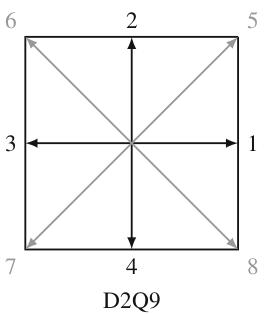
\includegraphics[width=.25\textwidth]{images/LB/D2Q9.png}
\caption{\small D2Q9 lattice set.}
\end{figure}
 
\begin{figure}
\centering
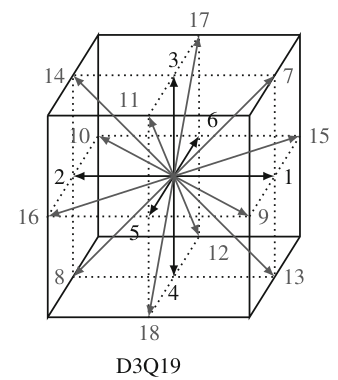
\includegraphics[width=0.26\textwidth]{images/LB/D3Q19.png}
\caption{\small D3Q19 lattice set.}
\end{figure}

For each velocities set there is a set of weights constants $\{\omega_i\}$ associated for each velocity, so that now we define a set of velocities and weights $\{\vec v_i,\omega_i\}$ which satisfies the following conditions:
\begin{subequations}\label{eqs:sums_vw}
\begin{equation}\label{eq:sum_wi}
    \sum_i \omega_i = 1
\end{equation}
\begin{equation}\label{eq:sum_viwi}
    \sum_i v_{i\alpha}\omega_i = 0
\end{equation}
\begin{equation}\label{eq:sum_viviwi}
    \sum_i v_{i\alpha}v_{i\beta}\omega_i = c_s^2\delta_{\alpha\beta}
\end{equation}
\begin{equation}\label{eq:sum_viviviwi}
    \sum_i v_{i\alpha}v_{i\beta}v_{i\gamma}\omega_i = 0
\end{equation}
\begin{equation}\label{eq:sum_viviviviwi}
    \sum_i v_{i\alpha}v_{i\beta}v_{i\gamma}v_{i\mu}\omega_i = c_s^4(\delta_{\alpha\beta}\delta_{\gamma\mu} + \delta_{\alpha\gamma}\delta_{\beta\mu} + \delta_{\alpha\mu}\delta_{\beta\gamma})
\end{equation}
\end{subequations}
Where $c_s^2$ is \textbf{for now a constant}.

In order to gather the PDE satisfied by the macroscopic moments defined at \ref{eqs:moments} we need to develop a \textbf{Chapman-Enskog analysis}. If the continuous transport Boltzmann equation is written as 
\begin{equation}\label{eq:C_LBE}
    \bigg(\partial_{t} + v_{i\alpha}\partial_\alpha\bigg)f_i = -\frac{\delta t}{\tau}(f_i - f^{\text{eq}})
\end{equation}
defining $\partial_t = \partial/\partial t$ and $\partial_\alpha = \partial/\partial x_\alpha$, a Taylor expansion is done in order to write
\begin{equation}\label{eq:LBE_taylor}
    \delta t\bigg(\partial_{t} + v_{i\alpha}\partial_\alpha\bigg)f_i + \frac{\delta t^2}{2!}\bigg(\partial_{t} + v_{i\alpha}\partial_\alpha\bigg)^2f_i + \mathcal{O}(\delta t^3) = -\frac{\delta t}{\tau}(f_i - f^{\text{eq}})
\end{equation}
expanding up to second order of $\delta t$. Identifying the Knusden number $\epsilon = \delta x/x$ %with $x$ the characteristic size of the system and $\delta x$ the size of a lattice cell,  
 we may develop a \textbf{perturbation expansion} for $f_i$ and the differential operators as follows:
\begin{subequations}\label{eq:exp_f}
    \begin{equation}
        f_i = f_i^{(0)} + \epsilon f_i^{(1)} + \epsilon^2 f_i^{(2)} + \dots
    \end{equation}
    \begin{equation}
        \partial_t = \epsilon \partial_t^{(1)} + \epsilon^2 \partial_t^{(2)} + \dots
    \end{equation}
    \begin{equation}
        \partial_\alpha = \epsilon \partial_\alpha^{(1)} + \dots
    \end{equation}
\end{subequations}

As the macroscopic moments must not be affected by the size of the lattice cells $\delta x$, these only contribute at order zero, thus one can write
\begin{equation}\label{eqs:moments_order_zero}
    \sum_i f_i^{(n)} = 0 \quad, \quad\sum_i v_{i\alpha}f_i^{(n)} = 0\quad\text{ if }\quad n>0
\end{equation}
Now replacing \ref{eq:exp_f} in \ref{eq:LBE_taylor} and neglecting the terms of higher orders of $\epsilon$ we have
\begin{align}
    &\epsilon^2\bigg\{\partial_t^{(2)}f_i^{(0)}+\left(\partial_t^{(1)}+v_{i\alpha}\partial_{\alpha}^{(1)}\right)f_i^{(1)}+\frac{\delta t}{2}\left(\partial_t^{(1)}+v_{i\alpha}\partial_\alpha^{(1)}\right)^2f_i^{(0)}\bigg\}+\dots\nonumber\\
    &\dots+\epsilon\bigg(\partial_t^{(1)}+v_{i\alpha}\partial_\alpha^{(1)}\bigg)f_i^{(0)} = -\frac{1}{\tau}\left(f_i^{(0)} - f_i^{\text{eq}} + \epsilon f_i^{(1)} + \epsilon^2f_i^{(2)}\right)
\end{align}

So that equaling terms of the same order of $\epsilon$ the following relations are reached:
\begin{subequations}\label{eqs:match_orders}
\begin{equation}\label{eq:match_ord0}
    f_i^{(0)} = f_i^{\text{eq}}
\end{equation}
\begin{equation}\label{eq:match_ord1}
    \bigg(\partial_t^{(1)}+v_{i\alpha}\partial_\alpha^{(1)}\bigg)f_i^{(0)} = -\frac{1}{\tau}f_i^{(1)}
\end{equation}
\begin{equation}\label{eq:match_ord2}
    \partial_t^{(2)}f_i^{(0)}+\left(\partial_t^{(1)}+v_{i\alpha}\partial_{\alpha}^{(1)}\right)f_i^{(1)}+\frac{\delta t}{2}\left(\partial_t^{(1)}+v_{i\alpha}\partial_\alpha^{(1)}\right)^2f_i^{(0)} =  -\frac{1}{\tau}f_i^{(2)}
\end{equation}
\end{subequations}
The third term of equation \ref{eq:match_ord2} may be rewritten using \ref{eq:match_ord1} this way:
\begin{align}
    \frac{\delta t}{2}\left(\partial_t^{(1)}+v_{i\alpha}\partial_\alpha^{(1)}\right)^2f_i^{(0)} &= \frac{\delta t}{2}\left(\partial_t^{(1)}+v_{i\alpha}\partial_\alpha^{(1)}\right)\left(\partial_t^{(1)}+v_{i\alpha}\partial_\alpha^{(1)}\right)f_i^{(0)} \nonumber\\
    &= -\frac{\delta t}{2\tau}\left(\partial_t^{(1)}+v_{i\alpha}\partial_\alpha^{(1)}\right)f_i^{(1)}
\end{align}
So that it is possible to rewrite \ref{eqs:match_orders} as

\begin{subequations}\label{eqs:match_orders_rewrite}
\begin{equation}\label{eq:match_ord0_rw}
    f_i^{(0)} = f_i^{\text{eq}}
\end{equation}
\begin{equation}\label{eq:match_ord1_rw}
    \bigg(\partial_t^{(1)}+v_{i\alpha}\partial_\alpha^{(1)}\bigg)f_i^{(0)} = -\frac{1}{\tau}f_i^{(1)}
\end{equation}
\begin{equation}\label{eq:match_ord2_rw}
    \partial_t^{(2)}f_i^{(0)}+\left(1-\frac{\delta t}{2\tau}\right)\left(\partial_t^{(1)}+v_{i\alpha}\partial_{\alpha}^{(1)}\right)f_i^{(1)} =  -\frac{1}{\tau}f_i^{(2)}
\end{equation}
\end{subequations}
In order to recover the PDE satisfied in the macroscopic limit for the zero-order tensor $\Pi$, a summation over $i$ must be developed in \ref{eq:match_ord1_rw} multiplied by $\epsilon$ and \ref{eq:match_ord2_rw} multiplied by $\epsilon^2$, then the equations are added. For \ref{eq:match_ord1_rw} we have 
\begin{equation}\label{eq:sum_i_f1}
    \epsilon\sum_i\bigg(\partial_t^{(1)}+v_{i\alpha}\partial_\alpha^{(1)}\bigg)f_i^{\text{eq}} = -\epsilon\frac{1}{\tau}\sum_if_i^{(1)}
\end{equation}
and taking into account \ref{eqs:moments_order_zero} the eq. \ref{eq:sum_i_f1} becomes ($v_{i\alpha}$ does not depend on $x_\alpha$)
\begin{align}\label{eq:continuity_order1}
    \epsilon\partial_t^{(1)}\sum_if_i^{\text{eq}}+\epsilon\partial_\alpha^{(1)}\sum_iv_{i\alpha}f_i^{\text{eq}} &= 0 \nonumber\\
    \epsilon\partial_t^{(1)}\Pi + \epsilon\partial_\alpha^{(1)}\Pi_{\alpha} &= 0
\end{align}

For \ref{eq:match_ord2_rw} also taking into account \ref{eqs:moments_order_zero} we have
\begin{align}\label{eq:continuity_order2}
    \epsilon^2\left(1-\frac{\delta t}{2\tau}\right)\sum_i\bigg(\partial_t^{(1)}+v_{i\alpha}\partial_\alpha^{(1)}\bigg)f_i^{(1)} + \epsilon^2\sum_i\partial_{t}^{(2)}f_i^{\text{eq}} &= -\epsilon\frac{1}{\tau}\sum_if_i^{(2)} \nonumber\\
    \epsilon^2\left(1-\frac{\delta t}{2\tau}\right)\left(\partial_t^{(1)}\sum_if_i^{(1)}+\partial_\alpha^{(1)}\sum_iv_{i\alpha}f_i^{(1)}\right) + \epsilon^2\partial_{t}^{(2)}\sum_if_i^{\text{eq}} &= 0 \nonumber\\
    \epsilon^2\partial_{t}^{(2)}\Pi &= 0
\end{align}
Therefor adding \ref{eq:continuity_order1} and \ref{eq:continuity_order2} the continuity equation is obtained for the zero-order and first-order moments taking into account \ref{eq:exp_f}
\begin{align}\label{eq:escalar_continuity}
    \left(\epsilon\partial_t^{(1)} + \epsilon^2\partial_t^{(2)}\right)\Pi + \epsilon\partial_\alpha^{(1)}\Pi_{\alpha} &= 0 \nonumber\\
    \partial_t\Pi + \partial_\alpha\Pi_\alpha &= 0
\end{align}

Now doing the same process but multiplying \ref{eq:match_ord1_rw} and \ref{eq:match_ord2_rw} by $v_{i\alpha}$ before adding over $i$ the following is obtained:
\begin{align}\label{eq:momentum_conserv1}
    \epsilon\partial_t^{(1)}\sum_iv_{i\alpha}f_i^{\text{eq}}+\epsilon\partial_\beta^{(1)}\sum_iv_{i\alpha}v_{i\beta}f_i^{\text{eq}} &= 0 \nonumber\\
    \epsilon\partial_t^{(1)}\Pi_\alpha + \epsilon\partial_\beta^{(1)}\Pi_{\alpha\beta} &= 0
\end{align}
and
\begin{equation}
    \epsilon^2\left(1-\frac{\delta t}{2\tau}\right)\left(\partial_t^{(1)}\sum_iv_{i\alpha}f_i^{(1)}+\partial_\beta^{(1)}\sum_iv_{i\alpha}v_{i\beta}f_i^{(1)}\right) + \epsilon^2\partial_{t}^{(2)}\sum_iv_{i\alpha}f_i^{\text{eq}} = 0
\end{equation}
where the following tensor at first order is defined as
\begin{equation}\label{eq:first_order_tensor}
    \Pi_{\alpha\beta}^{(1)} = \sum_iv_{i\alpha}v_{i\beta}f_i^{(1)}
\end{equation}
such that the following PDE equation is obtained:
\begin{equation}\label{eq:momentum_conserv2}
    \epsilon^2\left(1-\frac{\delta t}{2\tau}\right)\partial_\beta^{(1)}\left(\Pi_{\alpha\beta}^{(1)}\right) + \epsilon^2\partial_t^{(2)}\Pi_{\alpha} = 0
\end{equation}
Another relation for the tensor defined in \ref{eq:first_order_tensor} is found multiplying the equation \ref{eq:match_ord1_rw} by $v_{i\alpha}v_{i\beta}$ and adding it over $i$. By doing this the following is given:
\begin{equation}\label{eq:Pi_order_one_viscosity}
    \partial_t^{(1)}\Pi_{\alpha\beta} + \partial_{\gamma}^{(1)}\Pi_{\alpha\beta\gamma} = - \frac{1}{\tau}\Pi_{\alpha\beta}^{(1)}
\end{equation}
then adding \ref{eq:momentum_conserv1} and \ref{eq:momentum_conserv2} the resulting PDE is
\begin{equation}\label{eq:vector_PDE}
    \partial_\beta\Pi_{\alpha\beta} + \partial_t\Pi_\alpha = -\epsilon^2\left(1 - \frac{\delta t}{2\tau}\right)\partial_\beta^{(1)}\Pi_{\alpha\beta}^{(1)}
\end{equation}
noting that if $\tau = \delta t/2$ the right side of equation \ref{eq:vector_PDE} vanishes, giving a continuity equation for the tensors $\Pi_\alpha$ and $\Pi_{\alpha\beta}$ 
\begin{equation}\label{eq:vector_continuity}
    \partial_\beta\Pi_{\alpha\beta} + \partial_t\Pi_\alpha = 0
\end{equation}
and for $\Pi$ and $\Pi_\alpha$ there is the equation \ref{eq:escalar_continuity}. It has been shown that macroscopic moments satisfy a PDE written as the time-derivative o a tensor of given order plus the divergence of a higher order tensor is equal to zero. 

To see these equations as conservation laws (mass conservation or momentum conservation) we shall define the macroscopic moments in terms of fields with physical meaning. For example, in order to convert the equation \ref{eq:vector_continuity} to a NSE equation, we must define the following:
\begin{subequations}\label{eq:fluid_macroscopic_variables}
\begin{equation}\label{eq:density_momentum}
    \Pi \equiv \rho = \sum_i f_i \quad;\quad \Pi_\alpha \equiv \rho u_\alpha = \sum_i v_{i\alpha} f_i 
\end{equation}
\begin{equation}\label{eq:momentum_tensor}
    \Pi_{\alpha\beta} \equiv p\delta_{\alpha\beta} + \rho u_\alpha u_\beta = \sum_i v_{i\alpha}v_{i\beta} f_i
\end{equation}
\begin{equation}\label{eq:third_order_tensor}
    \Pi_{\alpha\beta\gamma} \equiv p(u_\alpha\delta_{\beta\gamma} + u_\beta\delta_{\alpha\gamma} + u_\gamma\delta_{\alpha\beta}) = \sum_i v_{i\alpha}v_{i\beta}v_{i\gamma} f_i
\end{equation}
\end{subequations}
considering the main macroscopic variables for a fluid such as the density $\rho$, the velocity $u_\alpha$ and the pressure $p$. Also, the tensor $\Pi_{\alpha\beta}$ has been identified as the \textbf{momentum flux density tensor}. Using eqn. \ref{eq:escalar_continuity} with \ref{eq:density_momentum} the continuity equation is given as
\begin{equation}\label{eq:continuity_rho_u}
    \partial_\alpha (\rho u_\alpha) + \partial_t \rho = 0
\end{equation}

Using eqn. \ref{eq:vector_PDE} with \ref{eq:momentum_tensor} the following is gotten:
\begin{equation}
    \partial_\alpha p + \partial_\beta(\rho u_\alpha u_\beta) + \partial_t (\rho u_\alpha) = -\left(1 - \frac{\delta t}{2\tau}\right)\left(\epsilon\partial_\beta^{(1)}\right)\left(\epsilon\Pi_{\alpha\beta}^{(1)}\right)
\end{equation}
where the tensor $\Pi_{\alpha\beta}^{(1)}$ is determined by \ref{eq:Pi_order_one_viscosity} using \ref{eq:fluid_macroscopic_variables}. Taking into account that for any variable $x$
\begin{equation}
    \partial_x(abc) = a\partial_x(bc) + b\partial_x(ac) - ab\partial_xc
\end{equation}
and doing some algebra that will not be shown here it is proven that 
\begin{equation}\label{eq:Pi_order_one_solution}
    \Pi_{\alpha\beta}^{(1)} = -\tau\left(p(\partial_\beta^{(1)}u_\alpha + \partial_\alpha^{(1)}u_\beta) - \partial_\gamma^{(1)}(\rho u_\alpha u_\beta u_\gamma)\right)
\end{equation}
And finally it is necessary to use an equation of state in order to relate the density and the pressure. In this case the ideal gas law will be used assuming a constant temperature for the fluid
\begin{equation}\label{eq:equation_state}
    p = RT\rho = c_s^2\rho
\end{equation}
where here we have identified $c_s = \sqrt{RT}$ which has \textit{velocity units}. 

Note that the last term of equation \ref{eq:Pi_order_one_solution} is cubic in the velocity, however it may be neglected as soon as $u^2 \ll c_s^2$ is fulfilled. Using the expression obtained by \ref{eq:Pi_order_one_solution} without the cubic term and replacing it into \ref{eq:vector_PDE} is possible to get
\begin{equation}\label{eq:NSE_fromLB}
    \partial_\beta(\rho u_\alpha u_\beta) + \partial_t(\rho u_\alpha) = -\partial_\alpha p + \eta\partial_\beta(\partial_\beta u_\alpha + \partial_\alpha u_\beta)
\end{equation}
with
\begin{equation}\label{eq:viscosity_tau_p}
    \eta = \rho c_s^2\left(\tau - \frac{\delta t}{2}\right)
\end{equation}
will be the viscosity. Is possible to see that for $\tau = \delta t/2$ we end up with the \textbf{Euler equation}. Although we have associated the moments from $f_i$ to physical quantities to get continuity and NSE equation in \ref{eq:fluid_macroscopic_variables}, this association is not possible if the equilibrium function $f_i^{\text{eq}}$ is not properly defined in terms of these physical quantities. The equilibrium function must be written such that is possible to retrieve all the macroscopic moments using \ref{eqs:moments}. 

One way to find the proper $f_i^{\text{eq}}$ is by \textbf{moment matching}. This consist of writing the equilibrium function as an \textit{ansatz} written as
\begin{equation}
    f_i^{\text{eq}} = \omega_i\rho(1 + a_1v_{i\alpha}u_\alpha + a_2v_{i\alpha}v_{i\beta}u_\alpha u_\beta - a_3u_\alpha u_\beta)
\end{equation}
where $\omega_i$ are the weights that complement the velocity set. Then the constants $a_1$, $a_2$ and $a_3$ are found such that using the conditions for $v_{i\alpha}$ and $\omega_i$ described in \ref{eqs:sums_vw} the macroscopic variables are obtained. For the case of fluids we have
\begin{equation}\label{eq:moment_matching_constants}
    a_1 = \frac{1}{c_s^2}\quad;\quad a_2 = \frac{1}{2c_s^4}\quad;\quad a_3 = \frac{1}{2c_s^2}
\end{equation}
where $c_s^2$ constant appears once again due to \ref{eqs:sums_vw}, but finding the second order tensor, after doing the math we find that this matches the momentum flux tensor
\begin{equation}
    \sum_i v_{i\alpha}v_{i\beta}f_i^{\text{eq}} = c_s^2\rho\delta_{\alpha\beta} + \rho u_{i\alpha}u_{i\beta} = \Pi_{\alpha\beta}
\end{equation}
thus, the constant $c_s^2$ appearing in \ref{eqs:sums_vw} matches with the $c_s^2$ of \ref{eq:equation_state} and $f_i^{\text{eq}}$ is
\begin{equation}
    f_i^{\text{eq}} = \omega_i\rho\left(1 + \frac{v_{i\alpha}u_\alpha}{c_s^2} + \frac{v_{i\alpha}v_{i\beta}u_\alpha u_\beta}{2c_s^4} - \frac{u_\alpha u_\beta}{2c_s^2}\right)
\end{equation}

\section{Chopard's original model}
The proposal of B. Chopard, P.O. Luthi and J. Wagen comes from a two-dimensional cellular automata composed by particles moving around a cartesian Lattice grid. To summarize the evolution rule we have a black particle connected to four white neighbour particles. 

If the position of the black particle is $\vec r_{i,j} = (x_{i,j},y_{i,j})$ and the position of each white neighbor particle is $\vec r_{i-1,j}$, $\vec r_{i+1,j}$, $\vec r_{i,j-1}$ and $\vec r_{i,j+1}$ the distances between the black particle and the white ones are
\begin{subequations}\label{eq:f_i_chopard}
\begin{equation}
    f_1(i,j,t) = x_{i-1,j}(t) - x_{i,j}(t)
\end{equation}
\begin{equation}
    f_2(i,j,t) = x_{i,j-1}(t) - x_{i,j}(t)
\end{equation}
\begin{equation}
    f_3(i,j,t) = x_{i+1,j}(t) - x_{i,j}(t)
\end{equation}
\begin{equation}
    f_4(i,j,t) = x_{i,j+1}(t) - x_{i,j}(t)
\end{equation}
\end{subequations}
To deduct the evolution rule easier, we consider the case where the black particle is at the origin, that is $x_{i,j}(t) = 0$, then the x-coordinate of the mass center of the white particles is simply
\begin{equation}
    X_{CM} = \frac{1}{4}(f_1 + f_2 + f_3 + f_4)
\end{equation}


then the black particle will try to oscillate around the center of mass $X_{CM}$, thus it will reach a symmetrical position with respect to the center of mass. This leads to
\begin{equation}
    x_{i,j}(t+1) = 2 X_{CM} = \frac{1}{2}(f_1 + f_2 + f_3 + f_4)
\end{equation}
while the white particles will move at the next step, we need to compute the distances written in \ref{eq:f_i_chopard} but respect to the position of each white particle
\begin{align}
    f_1(i+1,j,t+1) &= x_{i,j}(t+1) - x_{i+1,j}(t+1) \\
    &= 2 X_{CM} - x_{i+1,j}(t+1)
\end{align}
so that using \ref{eq:f_i_chopard} we may write 
\begin{align}
    f_1(i+1,j,t) &= \frac{1}{2}(f_1 + f_2 + f_3 + f_4) - f_3 \\
    &= \frac{1}{2}(f_1 + f_2 - f_3 + f_4)
\end{align}

Following a similar procedure for $f_2$, $f_3$ and $f_4$ the evolution rule may be written in the following matrix representation
\begin{equation}\label{eq:evolution_rule_waves}
    \begin{pmatrix}
        f_1(i+1,j,t+1) \\
        f_2(i,j+1,t+1) \\
        f_3(i-1,j,t+1) \\
        f_4(i,j-1,t+1) \\        
    \end{pmatrix}
    =
    \bm{W}\begin{pmatrix}
        f_1(i,j,t) \\
        f_2(i,j,t) \\
        f_3(i,j,t) \\
        f_4(i,j,t) \\        
    \end{pmatrix}
\end{equation}
defining the matrix 
\begin{equation}\label{eq:W_chopard_evolution_rule}
    \bm{W} = \frac{1}{2}\begin{pmatrix}
        1 & 1 & -1 & 1 \\
        1 & 1 & 1 & -1 \\
        -1 & 1 & 1 & 1 \\
        1 & -1 & 1 & 1 \\
    \end{pmatrix}
\end{equation}
Chopard have shown that with this cellular automata is possible to simulate waves propagation in two dimensions. Then he shows how to obtain a similar evolution rule using the Lattice-Boltzmann equation \ref{eq:LBE_BGK}. 
\begin{figure}
    \centering
    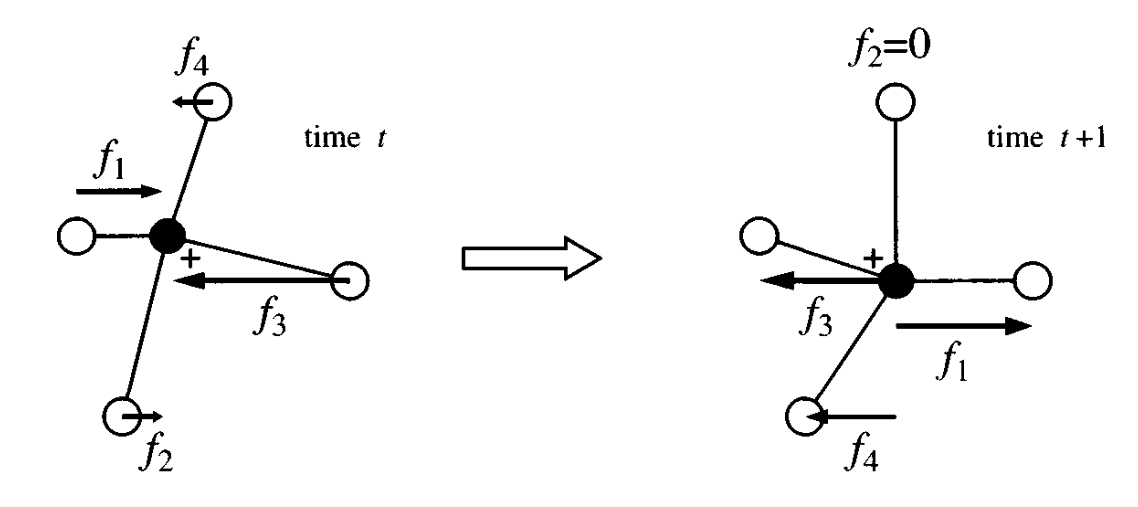
\includegraphics[width=0.7\textwidth]{images/LB/Chopard_2D_cellular_automata.png}
    \caption{Cellular automata scheme for 2D waves propagation.}
    \label{fig:chopard_2D_waves_cellular_automata}
\end{figure}

In order to reproduce the evolution rule written in \ref{eq:evolution_rule_waves} using \ref{eq:LBE_BGK} we define the following macroscopic variables:
\begin{equation}\label{eq:chopard_fields}
    \Psi = \sum_i f_i \quad;\quad J_{\alpha} = \sum_i v_{i\alpha}f_i
\end{equation}
where this time the velocity set is still D2Q5 but they fulfil the next relationships:
\begin{subequations}
\begin{equation}
    \sum_{i=0}^4 v_{i\alpha} = 0
\end{equation}
\begin{equation}
    \sum_{i=0}^4 v_{i\alpha}v_{i\beta} = 2v^2\delta_{\alpha\beta}
\end{equation}
\end{subequations}
where $v$ is the magnitude of every velocity vector, for D2Q5 $v=1$.

Defining $a_0$ and $a$ which satisfy
\begin{equation}
    a_0 + 4a = 1
\end{equation} 
The equilibrium function is then
\begin{equation}\label{eq:chopard_feq}
    f_i^{\text{eq}} = \begin{cases}
        a_0\Psi & i=0\\
        a\Psi + \frac{\vec v_i \cdot \vec J}{2v^2} & i\neq0 
    \end{cases}
\end{equation}
Now, if we plug in \ref{eq:chopard_feq} into the Lattice-Boltzmann evolution rule with the BGK collision operator \ref{eq:LBE_BGK} we have for $i=0$
\begin{align}
    f_0(\vec x, t + \delta t) &= \frac{1}{\tau}\left( (\tau - 1)f_0 + a_0\Psi \right) \nonumber\\
    &= \frac{1}{\tau}\left((a_0+\tau-1)f_0 + a_0(f_1+f_2+f_3+f_4)\right)
\end{align}
and for $i\neq0$
\begin{equation}\label{eq:chopard_waves_evolution_rule_f0}
    f_i(\vec x+\delta t\vec v_i, t + \delta t) = \frac{1}{\tau}\left( a\Psi + \frac{\vec v_i \cdot \vec J}{2v^2} + (\tau-1)f_i \right)
\end{equation}

and after plugging in \ref{eq:chopard_fields} and doing some algebra 
\begin{align}\label{eq:chopard_waves_evolution_rule_fi}
    f_i(\vec x+\delta t\vec v_i, t + \delta t) &= \frac{1}{\tau}\bigg(\left(a+\tau-\frac{1}{2}\right)f_i+\dots\nonumber\\
    &\dots+ a f_{i+1} + \left(a-\frac{1}{2}\right)f_{i+2} + a f_{i+3} + a f_0\bigg)
\end{align}
This evolution rule defined in \ref{eq:chopard_waves_evolution_rule_f0} and \ref{eq:chopard_waves_evolution_rule_fi} may also be written as the following matrix equation
\begin{equation}
    \begin{pmatrix}
        f_0(\vec x, t + \delta t) \\
        f_1(\vec x+\delta t\vec v_i, t + \delta t) \\
        f_2(\vec x+\delta t\vec v_i, t + \delta t) \\
        f_3(\vec x+\delta t\vec v_i, t + \delta t) \\
        f_4(\vec x+\delta t\vec v_i, t + \delta t) \\        
    \end{pmatrix}
    =
    \bm{W'}\begin{pmatrix}
        f_0(\vec x, t) \\
        f_1(\vec x, t) \\
        f_2(\vec x, t) \\
        f_3(\vec x, t) \\
        f_4(\vec x, t) \\        
    \end{pmatrix}
\end{equation}

where the matrix $\bm{W'}$ is written as
\begin{equation}
    \bm{W'} = \frac{1}{\tau}\begin{pmatrix}
        a_0 + \tau - 1 & a_0 & a_0 & a_0 & a_0 \\
        a & a + \tau - 1/2 & a & a - 1/2 & a \\
        a & a & a + \tau - 1/2 & a & a - 1/2 \\
        a & a - 1/2 & a & a + \tau - 1/2 & a \\
        a & a & a - 1/2 & a & a + \tau - 1/2 \\
    \end{pmatrix}
\end{equation}
the interesting about $\bm{W'}$ is that for $i\neq0$ and $a_0 = 0$ we get
\begin{equation}
    \bm{W'} = \frac{1}{\tau}\begin{pmatrix}
        \tau - 1 & 0 & 0 & 0 & 0 \\
        1/4 & \tau - 1/4 & 1/4 & -1/4 & 1/4 \\
        1/4 & 1/4 & \tau - 1/4 & 1/4 & -1/4 \\
        1/4 & -1/4 & 1/4 & \tau - 1/4 & 1/4 \\
        1/4 & 1/4 & -1/4 & 1/4 & \tau - 1/4 \\
    \end{pmatrix}
\end{equation}

Finally, if we chose $\tau=1/2$ the resulting matrix will be
\begin{equation}
    \bm{W'} = \frac{1}{2}\begin{pmatrix}
        -2 & 0 & 0 & 0 & 0 \\
        1 & 1 & 1 & -1 & 1 \\
        1 & 1 & 1 & 1 & -1 \\
        1 & -1 & 1 & 1 & 1 \\
        1 & 1 & -1 & 1 & 1 \\
    \end{pmatrix}
\end{equation}
which is similar to the matrix $\bm{W}$ written in equation \ref{eq:W_chopard_evolution_rule}. The LB model shown here solves the equations
\begin{subequations}
\begin{equation}
    \partial_t \Psi + \partial_\alpha J_\alpha = 0
\end{equation}
\begin{equation}
    \partial_t J_\alpha + \partial_\beta\Pi_{\alpha\beta} = 0
\end{equation}
\end{subequations}
where
\begin{equation}
    \Pi_{\alpha\beta} = 2av^2\Psi\delta_{\alpha\beta}
\end{equation}
matching also \ref{eq:escalar_continuity} and \ref{eq:vector_continuity} if $\tau=1/2$. 

The waves equation is easily obtained using a similar procedure as in \ref{eq:proc_waves_rho} or \ref{eq:proc_waves_p} getting
\begin{equation}
    \partial_t^2\Psi = 2av^2\nabla^2\Psi
\end{equation}
where the propagation speed is identified as $c\equiv v\sqrt{2a}$ which depends on the free parameter $a$. This lets to adjust the speed making possible to model various refraction indexes and describing inhomogeneous media. 
\begin{figure}
    \centering
    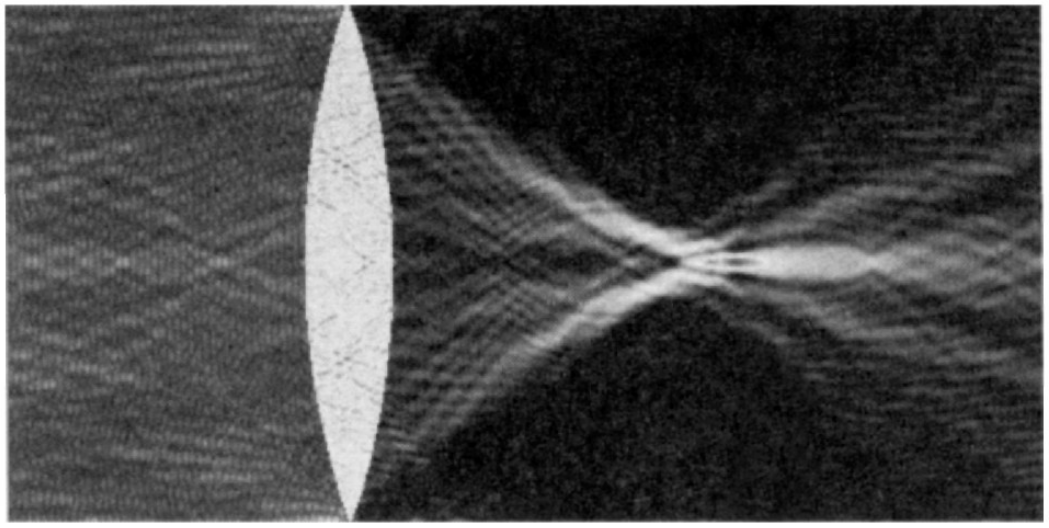
\includegraphics[width=0.4\textwidth]{images/LB/lens_LB_chopard.png}
    %\caption{Caption}
    \label{fig:lens}
\end{figure}
The Chopard's model solves the waves equation for a \textbf{generic scalar field} $\Psi$ with the help of an \textbf{auxiliary generic vector field} $\vec J$ regardless their physical meaning. \textit{However, if we want to adjust the speed we need to be careful of possible dependencies of $c$ in any of the fields.} 

As we have neglected the non-linear term $\rho u_{\alpha1}u_{\beta1}$ the momentum flux density tensor $\Pi_{\alpha\beta}$ has become the \textbf{diagonal} tensor
\begin{equation}
    \Pi_{\alpha\beta} = p_1\delta_{\alpha\beta} = c_s^2\rho_1\delta_{\alpha\beta}
\end{equation}
Therefor, if we want to use the Lattice-Boltzmann method to simulate the waves we shall use instead the following macroscopic variables
\begin{equation}
    \rho_1 = \sum_i f_i \quad;\quad \rho_0 u_{\alpha1} = \sum_i v_{i\alpha}f_i  \quad;\quad \Pi_{\alpha\beta} = p_1\delta_{\alpha\beta} = \sum_i v_{i\alpha}v_{i\beta}f_i
\end{equation}
and the equilibrium function that produces these macroscopic quantities is simply
\begin{equation}\label{eq:eq_function_waves_from_fluids}
    f_i^{\text{eq}} = \rho_1\omega_i + \rho_0\omega_i\frac{v_{i\alpha}u_{\alpha1}}{c_s^2}
\end{equation}
coinciding with the equilibrium function for fluids without the quadratic terms of velocity. 

The issue with this model is that $c_s^2$ comes from the conditions defined in \ref{eqs:sums_vw} which involve the velocities and weights set. If we want to change $c_s^2$ we need then to modify the weights such that \ref{eqs:sums_vw} still hold. Taking a lattice as D2Q5, \textbf{where only the first four equations of \ref{eqs:sums_vw} are satisfied}, we have:
\begin{equation}
    \{\vec v_i\} = \left\{\begin{bmatrix}
        0 \\
        0
    \end{bmatrix};\begin{bmatrix}
        1 \\
        0
    \end{bmatrix};\begin{bmatrix}
        0 \\
        1
    \end{bmatrix};\begin{bmatrix}
        -1 \\
        0
    \end{bmatrix};\begin{bmatrix}
        0 \\
        -1
    \end{bmatrix}\right\}
\end{equation}
and the weights are determined by \ref{eqs:sums_vw}, such that for \ref{eq:sum_wi} we have
\begin{equation}\label{eq:weights_first}
    \sum_i \omega_i = \omega_0 + \omega_1 + \omega_2 + \omega_3 + \omega_4 = 1
\end{equation}
for equation \ref{eq:sum_viwi},
\begin{align}
    \sum_i v_{x}\omega_i = \omega_1 - \omega_3 = 0\quad&\text{and}\quad\sum_i v_{y}\omega_i = \omega_2 - \omega_4 = 0 \nonumber\\
    \omega_1 = \omega_3\quad&\text{and}\quad\omega_2 = \omega_4 \label{eq:weights_second}
\end{align}

and for equation \ref{eq:sum_viviwi} 
\begin{align}
    \sum_i v_{x}v_{x}\omega_i = \omega_1 + \omega_3 = c_s^2\quad&\text{and}\quad\sum_i v_{y}v_{y}\omega_i = \omega_2 + \omega_4 = c_s^2 \nonumber\\
    \omega_1 = \frac{c_s^2}{2}\quad&\text{and}\quad\omega_2 = \frac{c_s^2}{2} \nonumber\\
    \sum_i v_{x}v_{y}\omega_i = 0 \quad&\text{and}\quad\sum_i v_{y}v_{x}\omega_i = 0 \label{eq:weights_third}
\end{align}
And replacing \ref{eq:weights_second} and \ref{eq:weights_third} into \ref{eq:weights_first} we end up with $i\neq0$
\begin{align}
    \omega_i &= \frac{c_s^2}{2} \label{eq:weight0_solution}\\
    \omega_0 &= 1 - 4\omega_i = 1 - 2c_s^2\label{eq:weights_solution}
\end{align}
which is consistent with the case $c_s = 1/\sqrt{3}$, $\omega_0 = 1/3$ and $\omega_i = 1/6$. Note that this only works for D2Q5.

Using this results the equilibrium function written in \ref{eq:eq_function_waves_from_fluids} will take the form
\begin{equation}
    f_i^{\text{eq}} = \begin{cases}
        (1 - 2 c_s^2)\rho_1 = \omega_0\rho_1 & i=0 \\
        \frac{c_s^2}{2}\rho_1 + \frac{v_{i\alpha}(\rho_0 u_\alpha)}{2} = \omega_i\rho_1 + \frac{v_{i\alpha}(\rho_0 u_\alpha)}{2} & i\neq0 \\
    \end{cases} 
\end{equation}
now from \ref{eq:weight0_solution} and \ref{eq:weights_solution} of the D2Q5 lattice, equation \ref{eqs:sums_vw} becomes simply
\begin{subequations}\label{eqs:sums_vw}
\begin{equation}\label{eq:sum_wi_waves}
    \omega_0 + 4\omega_i = 1
\end{equation}
\begin{equation}\label{eq:sum_viwi_waves}
    \sum_i v_{i\alpha}\left(\frac{c_s^2}{2}\right) = 0
\end{equation}
\begin{equation}\label{eq:sum_viviwi_waves}
    \sum_i v_{i\alpha}v_{i\beta}\left(\frac{c_s^2}{2}\right) = c_s^2\delta_{\alpha\beta}
\end{equation}
\begin{equation}\label{eq:sum_viviviwi_waves}
    \sum_i v_{i\alpha}v_{i\beta}v_{i\gamma}\left(\frac{c_s^2}{2}\right) = 0
\end{equation}
\end{subequations}

Notice that \ref{eq:sum_viwi_waves} and \ref{eq:sum_viviwi_waves} become
\begin{subequations}
\begin{equation}\label{eq:sum_viwi_waves}
    \sum_i v_{i\alpha}= 0
\end{equation}
\begin{equation}\label{eq:sum_viviwi_waves}
    \sum_i v_{i\alpha}v_{i\beta} = 2\delta_{\alpha\beta}
\end{equation}
\end{subequations}
Such that once 

\chapter{Implementation of Lattice Boltzmann method for waves in LB3D}



%\part{ Proyecto de investigación}
\chapter{Acoustic radiation force over a cylinder and a sphere}

\chapter{Simulation of the acoustic radiation force on a cylinder and a sphere}
\chapter{Acoustic torque over a rotor in 2D}
\section{Symmetric case}

\section{Asymmetric case}
%\include{chap7_resultados_Pincer.tex}
%\include{chap7_resultados_Salen.tex}

\addcontentsline{toc}{chapter}{Conclusiones}
\chapter*{Conclusiones}


\printbibliography

%\appendix
%\addcontentsline{toc}{chapter}{Apéndices}
\chapter{Reporte de valores numéricos completos}\label{ap2}

\begin{table}[h]
\centering
\caption{Parámetros obtenidos de área superficial polar topológica (TPSA) y coeficiente de partición octanol-agua (logP) en las regresiones multilineales de ajuste de la permeación logBB a los descriptores moleculares. Contraste entre el método de Clark (ClogP, MlogP), Chaparro (XlogP) y el empleado en el presente estudio (milogP).}
\begin{tabular}{ccccc}
\hline
\textbf{Parámetro} & \textbf{ClogP} & \textbf{MlogP} & \textbf{XlogP} & \textbf{milogP} \\ \hline
TPSA               & -0,0148          & -0,0145          & -0,0106         & -0,0146          \\
logP              & 0,152            & 0,172            & 0,156           & 0,167            \\
Intercepto         & 0,139            & 0,131            & 0,053           & 0,113            \\
R$^{2}$                 & 0,778            & 0,759            & 0,711           & 0,756            \\
Desv. Est          & 0,354            & 0,369            & 0,404           & 0,371            \\
F                  & 95,84            & 86,01            & 67,35           & 84,64            \\
Crit. F            & 3,62E-18         & 3,23E-17         & 3,68E-15        & 4,44E-17         \\ \hline
\end{tabular}
\end{table}

\clearpage

\hspace{0cm}
\vfill
\begin{figure}[ht] 
\centering
\includegraphics[scale=0.20]{images/cal_referencias.png}
\caption{Estructuras 2D de los ligandos empleados en el modelado de los 18 complejos de referencia (C) usados durante el proceso de calibración. Todas las vacancias fueron ocupadas con una relación M-L 1:2, excepto para el caso del complejo tridentado \textbf{C10} donde la cuarta vacancia fue ocupada con una molécula de agua. El \textbf{C14} se trata de un complejo de ácido 2-aminopropanoico y 1,10-fenantrolina.}
\label{cal_referencias}
\end{figure}
\vfill
\hspace{0cm}

\clearpage

\clearpage

\begin{table}[h]
\centering
\caption{Valores calculados de coeficiente de partición octanol-agua (milogP), área superficial polar topológica (TPSA), número de átomos donadores de enlace de hidrógeno (nON), número de grupos aceptores de enlace de hidrógeno (nOHNH) y peso molecular en unidades de masa atómicas (PM); y valores calculados de permeación de la BHE (logBB) para el conjunto de estudio de ligandos con átomos donadores de N, O y S.}
\begin{tabular}{c|ccccc|c}
\hline
\textbf{Ligando} & \textbf{milogP} & \textbf{TPSA} & \textbf{nON} & \textbf{nOHNH} & \textbf{PM} & \textbf{logBB} \\ \hline
1                & -2,09            & 48,11         & 4            & 4              & 172,28      & -0,94          \\
2                & -4,53            & 92,34         & 7            & 3              & 306,39      & -1,99          \\
3                & -4,36            & 136,57        & 10           & 2              & 440,50      & -2,61          \\
4                & -1,55            & 48,11         & 4            & 4              & 200,33      & -0,85          \\
5                & 0,48             & 63,73         & 7            & 2              & 390,58      & -0,74          \\
6                & -4,14            & 92,34         & 7            & 3              & 334,44      & -1,93          \\
7                & -3,89            & 136,57        & 10           & 2              & 468,56      & -2,53          \\
8                & 0,33             & 24,92         & 2            & 1              & 122,17      & -0,20          \\
9                & 0,34             & 49,84         & 4            & 2              & 242,33      & -0,56          \\
10               & 0,03             & 73,51         & 6            & 2              & 232,34      & -0,96          \\
11               & 0,92             & 73,51         & 6            & 2              & 260,39      & -0,81          \\
12               & 2,40             & 28,49         & 3            & 0              & 225,29      & 0,10           \\
13               & 2,12             & 28,16         & 3            & 1              & 227,31      & 0,06           \\
14               & 2,02             & 24,92         & 2            & 1              & 184,24      & 0,09           \\
15               & 1,10             & 50,94         & 3            & 3              & 199,26      & -0,45          \\
16               & 2,06             & 43,39         & 4            & 1              & 244,29      & -0,18          \\
17               & 3,37             & 28,16         & 3            & 1              & 277,37      & 0,26           \\
18               & 3,10             & 48,38         & 4            & 2              & 293,37      & -0,08          \\
19               & 3,38             & 37,39         & 4            & 1              & 307,40      & 0,13           \\
20               & 3,38             & 48,72         & 4            & 1              & 291,35      & -0,03          \\
21               & 3,66             & 37,73         & 4            & 0              & 305,38      & 0,17           \\
22               & 2,58             & 68,61         & 5            & 3              & 323,40      & -0,46          \\
23               & 2,81             & 40,77         & 4            & 1              & 253,31      & -0,01          \\
24               & 2,10             & 33,44         & 4            & 0              & 238,29      & -0,02          \\
25               & 3,13             & 33,44         & 4            & 0              & 364,19      & 0,15           \\
26               & 3,97             & 45,48         & 3            & 1              & 254,31      & 0,11           \\
27               & 4,62             & 45,48         & 3            & 1              & 288,76      & 0,22           \\
28               & 3,90             & 91,31         & 6            & 1              & 299,31      & -0,57          \\
29               & 4,44             & 46,26         & 3            & 1              & 337,12      & 0,18           \\
30               & 5,08             & 33,12         & 2            & 1              & 353,18      & 0,48           \\
31               & 4,04             & 54,71         & 3            & 3              & 335,15      & -0,01          \\ \hline
\end{tabular}
\end{table}

\clearpage

\begin{table}[h]
\centering
\caption{Valores calculados de coeficiente de partición octanol-agua (milogP), área superficial polar topológica (TPSA), número de átomos donadores de enlace de hidrógeno (nON), número de grupos aceptores de enlace de hidrógeno (nOHNH) y peso molecular en unidades de masa atómicas (PM); y valores calculados de permeación de la BHE (logBB) para el conjunto de estudio de ligandos tipo pinza.}
\begin{tabular}{c|ccccc|c}
\hline
\textbf{Ligando} & \textbf{milogP} & \textbf{TPSA} & \textbf{nON} & \textbf{nOHNH} & \textbf{PM} & \textbf{logBB} \\ \hline
32               & 4,45             & 67,70         & 6            & 0              & 370,51      & -0,13           \\
33               & 2,43             & 108,15        & 8            & 2              & 402,50      & -1,06           \\
34               & 3,40             & 52,48         & 3            & 3              & 201,22      & -0,09           \\
35               & 4,24             & 52,48         & 3            & 3              & 229,28      & 0,05            \\
36               & 3,67             & 52,48         & 3            & 3              & 237,21      & -0,04           \\
37               & 4,96             & 52,48         & 3            & 3              & 359,02      & 0,18            \\
38               & 8,96             & 12,03         & 1            & 1              & 537,58      & 1,43            \\
39               & 9,24             & 12,03         & 1            & 1              & 565,64      & 1,48            \\
40               & 9,06             & 12,03         & 1            & 1              & 573,56      & 1,45            \\
41               & 9,43             & 12,03         & 1            & 1              & 695,38      & 1,51            \\
42               & 7,82             & 36,08         & 3            & 3              & 351,45      & 0,89            \\
43               & 8,51             & 36,08         & 3            & 3              & 379,51      & 1,01            \\
44               & 8,09             & 36,08         & 3            & 3              & 387,43      & 0,94            \\
45               & 8,87             & 36,08         & 3            & 3              & 509,25      & 1,07            \\
46               & 7,24             & 40,52         & 3            & 1              & 401,51      & 0,73            \\
47               & 9,01             & 40,52         & 3            & 1              & 485,68      & 1,03            \\
48               & 8,97             & 40,52         & 3            & 1              & 485,68      & 1,02            \\
49               & 9,64             & 40,52         & 3            & 1              & 569,84      & 1,13            \\
50               & 6,67             & 36,95         & 3            & 2              & 477,49      & 0,69            \\
51               & 8,35             & 12,89         & 1            & 0              & 555,64      & 1,32            \\
52               & 4,80             & 37,62         & 3            & 0              & 313,40      & 0,37            \\
53               & 3,39             & 38,68         & 3            & 0              & 275,36      & 0,11            \\
54               & 4,68             & 38,15         & 3            & 0              & 301,39      & 0,34            \\
55               & 5,52             & 25,78         & 2            & 0              & 390,43      & 0,66            \\
56               & 5,70             & 3,24          & 1            & 0              & 441,58      & 1,02            \\
57               & 6,06             & 9,23          & 1            & 0              & 442,56      & 0,99            \\
58               & 4,36             & 12,89         & 1            & 0              & 395,55      & 0,65            \\
59               & 7,07             & 31,36         & 3            & 0              & 479,46      & 0,84            \\
60               & 1,78             & 59,40         & 5            & 1              & 239,28      & -0,46           \\
61               & 3,68             & 43,08         & 4            & 0              & 290,37      & 0,10            \\
62               & 5,48             & 25,78         & 2            & 0              & 382,45      & 0,65            \\
63               & 4,35             & 25,26         & 2            & 0              & 412,41      & 0,47            \\
64               & 8,49             & 12,89         & 1            & 0              & 575,63      & 1,34            \\
65               & 4,37             & 45,48         & 3            & 1              & 288,35      & 0,18            \\ \hline
\end{tabular}
\end{table}

\clearpage

\begin{table}[h]
\centering
\caption{Valores calculados de coeficiente de partición octanol-agua (milogP), área superficial polar topológica (TPSA), número de átomos donadores de enlace de hidrógeno (nON), número de grupos aceptores de enlace de hidrógeno (nOHNH) y peso molecular en unidades de masa atómicas (PM); y valores calculados de permeación de la BHE (logBB) para el conjunto de estudio de ligandos tipo salen (primera parte).}
\begin{tabular}{c|ccccc|c}
\hline
\textbf{Ligando} & \textbf{milogP} & \textbf{TPSA} & \textbf{nON} & \textbf{nOHNH} & \textbf{PM} & \textbf{logBB} \\ \hline
1A               & 3,11             & 65,18         & 4            & 2              & 268,32      & -0,32          \\
1B               & 4,30             & 65,18         & 4            & 2              & 324,42      & -0,12          \\
1C               & 6,48             & 65,18         & 4            & 2              & 380,53      & 0,24           \\
1D               & 8,85             & 65,18         & 4            & 2              & 492,75      & 0,64           \\
1E               & 3,96             & 65,18         & 4            & 2              & 337,21      & -0,18          \\
1F               & 5,22             & 65,18         & 4            & 2              & 406,10      & 0,03           \\
1G               & 2,32             & 83,55         & 6            & 2              & 328,37      & -0,72          \\
1H               & -0,38            & 169,28        & 8            & 10             & 328,38      & -2,42          \\
1I               & 5,43             & 65,18         & 4            & 2              & 368,44      & 0,07           \\
1J               & 0,89             & 50,51         & 4            & 0              & 238,29      & -0,48          \\
1K               & 1,54             & 56,31         & 4            & 2              & 214,27      & -0,45          \\
2A               & 3,38             & 65,18         & 4            & 2              & 282,34      & -0,27          \\
2B               & 4,57             & 65,18         & 4            & 2              & 338,45      & -0,08          \\
2C               & 6,75             & 65,18         & 4            & 2              & 394,56      & 0,29           \\
2D               & 8,96             & 65,18         & 4            & 2              & 506,77      & 0,66           \\
2E               & 4,23             & 65,18         & 4            & 2              & 351,23      & -0,13          \\
2F               & 5,49             & 65,18         & 4            & 2              & 420,12      & 0,08           \\
2G               & 2,59             & 83,65         & 6            & 2              & 342,39      & -0,68          \\
2H               & -0,10            & 169,28        & 8            & 10             & 342,40      & -2,38          \\
2I               & 5,70             & 65,18         & 4            & 2              & 382,46      & 0,11           \\
2J               & 1,16             & 50,51         & 4            & 0              & 252,32      & -0,43          \\
2K               & 1,81             & 56,31         & 4            & 2              & 228,30      & -0,41          \\ \hline
\end{tabular}
\end{table}

\clearpage

\begin{table}[h]
\centering
\caption{Valores calculados de coeficiente de partición octanol-agua (milogP), área superficial polar topológica (TPSA), número de átomos donadores de enlace de hidrógeno (nON), número de grupos aceptores de enlace de hidrógeno (nOHNH) y peso molecular en unidades de masa atómicas (PM); y valores calculados de permeación de la BHE (logBB) para el conjunto de estudio de ligandos tipo salen (segunda parte).}
\begin{tabular}{c|ccccc|c}
\hline
\textbf{Ligando} & \textbf{milogP} & \textbf{TPSA} & \textbf{nON} & \textbf{nOHNH} & \textbf{PM} & \textbf{logBB} \\ \hline
3A               & 3,66             & 65,18         & 4            & 2              & 296,37      & -0,23          \\
3B               & 4,84             & 65,18         & 4            & 2              & 352,48      & -0,03          \\
3C               & 7,02             & 65,18         & 4            & 2              & 408,59      & 0,33           \\
3D               & 9,06             & 65,18         & 4            & 2              & 520,80      & 0,67           \\
3E               & 4,50             & 65,18         & 4            & 2              & 365,26      & -0,09          \\
3F               & 5,76             & 65,18         & 4            & 2              & 434,15      & 0,12           \\
3G               & 2,86             & 83,65         & 6            & 2              & 356,42      & -0,63          \\
3H               & 0,17             & 169,28        & 8            & 10             & 356,43      & -2,33          \\
3I               & 5,97             & 65,18         & 4            & 2              & 396,49      & 0,16           \\
3J               & 1,43             & 50,51         & 4            & 0              & 266,35      & -0,39          \\
3K               & 2,08             & 56,31         & 4            & 2              & 242,33      & -0,36          \\
4A               & 4,84             & 65,18         & 4            & 2              & 316.36      & -0,03          \\
4B               & 6,02             & 65,18         & 4            & 2              & 372.47      & 0,17           \\
4C               & 8,18             & 65,18         & 4            & 2              & 428.58      & 0,53           \\
4D               & 9,40             & 65,18         & 4            & 2              & 540.79      & 0,73           \\
4E               & 5,68             & 65,18         & 4            & 2              & 385.25      & 0,11           \\
4F               & 6,94             & 65,18         & 4            & 2              & 454.14      & 0,32           \\
4G               & 4,04             & 83,65         & 6            & 2              & 376.41      & -0,43          \\
4H               & 1,35             & 169,28        & 8            & 10             & 376.42      & -2,13          \\
4I               & 7,16             & 65,18         & 4            & 2              & 416.48      & 0,36           \\
4J               & 2,61             & 50,51         & 4            & 0              & 286.34      & -0,19          \\
4K               & 3,26             & 56,31         & 4            & 2              & 262.32      & -0,16          \\ \hline
\end{tabular}
\end{table}

\clearpage

\begin{table}[h]
\centering
\caption{Valores calculados de SRP (V) y afinidad para el conjunto de estudio de ligandos con átomos donadores de N, O y S.}
\begin{tabular}{cccc}
\hline
\textbf{Ligando} & \textbf{SRP} & \textbf{log $\boldsymbol{\beta$ $Cu^{1+}}$} & \textbf{log $\boldsymbol{\beta$ $Cu^{2+}}$} \\ \hline
\multicolumn{4}{c}{\textbf{Complejos en relación 1:2}}                         \\ \hline
1                & -0,38        & 9,54                 & 21,33                 \\
2                & -0,16        & 16,50                & 30,75                 \\
3                & 0,11         & 18,33                & 23,24                 \\
4                & -0,95        & 5,28                 & 26,67                 \\
5                & -0,44        & 17,08                & 31,27                 \\
6                & -0,33        & 21,80                & 38,94                 \\
7                & -0,64        & 14,31                & 30,42                 \\
8                & 0,17         & 9,55                 & 18,20                 \\
9                & 0,23         & 12,55                & 20,20                 \\
10               & 0,59         & 15,12                & 12,09                 \\
11               & 0,52         & 16,20                & 14,37                 \\
12               & 0,57         & 7,86                 & 9,68                  \\
13               & -0,61        & -37,56               & -15,83                \\
14               & -0,70        & -32,21               & -13,60                \\
15               & -0,56        & -37,20               & -16,33                \\
16               & -0,38        & -32,23               & -14,35                \\
19               & -0,62        & -34,99               & -13,07                \\
22               & -0,09        & -6,40                & 5,41                  \\
23               & -0,20        & 3,21                 & 2,06                  \\
24               & 0,00         & 5,01                 & 10,68                 \\
26               & -0,20        & -10,82               & -2,12                 \\
28               & 0,55         & -1,46                & -0,46                 \\ \hline
\multicolumn{4}{c}{\textbf{Complejos en relación 1:1}}                         \\ \hline
8                & 0,25         & 5,70                 & 8,34                  \\
15               & -0,05        & -16,23               & -8,62                 \\
16               & 0,01         & -14,00               & -7,42                 \\
26               & 0,14         & -4,51                & -0,05                 \\
27               & 0,09         & -6,27                & -1,03                 \\
28               & 0,23         & -2,01                & 0,83                  \\ \hline
\end{tabular}
\end{table}

\clearpage

\begin{table}[h]
\centering
\caption{Valores calculados de SRP (V) y afinidad para el conjunto de estudio de ligandos tipo pincer.}
\begin{tabular}{c|ccc}
\hline
\textbf{Ligando} & \textbf{SRP} & \textbf{log $\boldsymbol{\beta$ $Cu^{1+}}$} & \textbf{log $\boldsymbol{\beta$ $Cu^{2+}}$} \\ \hline
32               & 0,58             & -3,23                & -6,16                 \\
33               & 0,64             & -4,13                & -8,14                 \\
43               & -0,09            & -12,91               & -4,65                 \\
44               & 0,05             & -11,12               & -5,19                 \\
46               & -0,17            & -5,60                & 4,09                  \\
47               & -0,18            & -6,40                & 3,36                  \\
48               & -0,24            & -5,29                & 5,57                  \\
49               & -0,43            & -7,42                & 6,60                  \\
50               & 0,82             & 3,99                 & -3,15                 \\
51               & 1,03             & -2,18                & -12,87                \\
52               & 0,07             & 2,66                 & 8,34                  \\
53               & -0,03            & 6,81                 & 14,20                 \\
54               & 0,12             & 6,64                 & 11,40                 \\
55               & 0,35             & 2,98                 & 3,81                  \\
56               & 1,04             & 8,35                 & -2,50                 \\
57               & 1,03             & 10,49                & -0,17                 \\
58               & 0,27             & 9,76                 & 11,97                 \\
59               & 1,09             & 1,03                 & -10,51                \\
60               & 0,28             & 4,31                 & 6,32                  \\
61               & 0,19             & 5,24                 & 8,84                  \\
62               & 0,28             & 5,56                 & 7,60                  \\
63               & 0,43             & 3,13                 & 2,72                  \\
64               & 1,57             & 6,40                 & -13,26                \\
65               & -0,35            & -0,95                & 11,78                 \\ \hline
\end{tabular}
\end{table}

\clearpage

\begin{table}[h]
\centering
\caption{Valores calculados de SRP (V) y afinidad para el conjunto de estudio de ligandos tipo salen (primera parte).}
\begin{tabular}{c|ccc}
\hline
\textbf{Ligando} & \textbf{SRP} & \textbf{log $\boldsymbol{\beta$ $Cu^{1+}}$} & \textbf{log $\boldsymbol{\beta$ $Cu^{2+}}$} \\ \hline
1A               & -0,81        & -5,86                & 18,13                 \\
1B               & -0,86        & -7,87                & 16,97                 \\
1C               & -0,82        & -7,78                & 16,36                 \\
1D               & -0,62        & -7,66                & 13,06                 \\
1E               & -0,71        & -3,31                & 18,93                 \\
1F               & -0,61        & -3,03                & 17,55                 \\
1G               & -0,81        & -8,06                & 15,98                 \\
1H               & -0,88        & -7,46                & 17,80                 \\
1I               & -0,76        & -9,02                & 14,17                 \\
1J               & 0,45         & 7,50                 & 11,36                 \\
1K               & -0,56        & -13,59               & 2,73                  \\
2A               & -0,67        & -5,61                & 15,98                 \\
2B               & -0,77        & -9,01                & 14,26                 \\
2C               & -0,70        & -7,84                & 14,25                 \\
2D               & -0,80        & -6,69                & 17,20                 \\
2E               & -0,58        & -3,90                & 16,15                 \\
2F               & -0,49        & -3,50                & 15,04                 \\
2G               & -0,71        & -8,64                & 13,62                 \\
2H               & -0,78        & -9,13                & 14,37                 \\
2I               & -0,64        & -8,85                & 12,25                 \\
2J               & 0,95         & 7,96                 & 3,31                  \\
2K               & -0,81        & -11,56               & 8,97                  \\ \hline
\end{tabular}
\end{table}

\clearpage

\begin{table}[h]
\centering
\caption{Valores calculados de SRP (V) y afinidad para el conjunto de estudio de ligandos tipo salen (segunda parte).}
\begin{tabular}{c|ccc}
\hline
\textbf{Ligando} & \textbf{SRP} & \textbf{log $\boldsymbol{\beta$ $Cu^{1+}}$} & \textbf{log $\boldsymbol{\beta$ $Cu^{2+}}$} \\ \hline
3A               & -0,57        & -6,10                & 13,89                 \\
3B               & -0,61        & -6,85                & 13,79                 \\
3C               & -0,62        & -7,95                & 12,79                 \\
3D               & -0,73        & -6,54                & 16,10                 \\
3E               & -0,49        & -3,56                & 15,07                 \\
3F               & -0,39        & -4,03                & 12,85                 \\
3G               & -0,57        & -7,48                & 12,49                 \\
3H               & -0,67        & -7,50                & 14,13                 \\
3I               & -0,53        & -7,25                & 12,08                 \\
3J               & 0,47         & 9,32                 & 12,89                 \\
3K               & -0,68        & -12,09               & 6,15                  \\
4A               & -0,72        & -4,01                & 18,48                 \\
4B               & -0,79        & -5,67                & 17,98                 \\
4C               & -0,75        & -6,79                & 16,26                 \\
4D               & -0,70        & -3,13                & 19,01                 \\
4E               & -0,62        & -2,24                & 18,52                 \\
4F               & -0,54        & -2,80                & 16,65                 \\
4G               & -0,77        & -6,16                & 17,20                 \\
4H               & -0,76        & -5,01                & 18,21                 \\
4I               & -0,71        & -7,02                & 15,24                 \\
4J               & 0,49         & 8,01                 & 11,14                 \\
4K               & -0,69        & -11,45               & 6,96                  \\ \hline
\end{tabular}
\end{table}
%\chapter{Estudio de los modos de coordinación}\label{ap1}

Para el estudio de la coordinación de los ligandos que lo requerían se consideraron todos los modos posibles que guardan sentido químico y se modelaron con el método DFT expuesto en la metodología de trabajo. Como fue mencionado en el preámbulo del capítulo \ref{cap_resultados}, hay algunos resultados para los ligandos que sufrieron dos complicaciones derivadas del que disminuyeron el número de candidatos a evaluar debido a la imposibilidad de obtener valores de energía libre confiables para algunos de sus modos de coordinación. Por lo anterior, se decidió emplear un código de identificación en este apéndice para marcar si una estructura dada involucra alguno de estos dos problemas. Así, en las figuras de las secciones a continuación se indica que se obtuvo como resultado una \textbf{reducción parcial del cobre} mediante un \textbf{círculo de color amarillo} sobre la carga del complejo en cuestión, mientras que un \textbf{cambio de energía anómalo en la corrección SP} se indica con una \textbf{carga subrayada y en negrilla}. 

\section{Ligandos con átomos donadores de N, O y S}

A continuación se presentan las estructuras 2D de los modos resultantes junto con las interacciones no covalentes más importantes para cada caso, indicando la estructura que resulta ser más estable termodinámicamente en color verde y omitiendo del análisis a las moléculas que involucran resultados inconsistentes marcadas con el código de identificación.

\subsection{Derivados tetraazamacrocíclicos}

Las Figs. \ref{estcoord_1_3} y \ref{estcoord_4_7} muestran que la desprotonación de los anillos en los derivados tetraazamacrocíclicos da lugar a deltas de energía libre positivos en todos los casos para los complejos formados con ambos cationes $Cu^{1+}$ y $Cu^{2+}$, por lo que las estructuras más estables resultan ser aquellas con anillos completamente protonados. Se observa también que añadir un metilpicolinato a la estructura \textbf{1} original hace que los modos de coordinación más estables para ambos cationes de cobre cambien de 4N a 5N para el ligando \textbf{2}, lo que ocurre gracias a la coordinación del anillo de piridina del fragmento el cual a su vez induce una geometría piramidal. Por otro lado, añadir un segundo metilpicolinato en el amino opuesto como sucede con la estructura \textbf{3} modifica la coordinación con el $Cu^{1+}$ a un modo 3N1O, incluyendo a un oxígeno del grupo carboxilato en la coordinación y rompiendo las interacciones del metal con los aminos sustituidos.\\

Respecto a los macrociclos de más miembros, encontramos que el ligando \textbf{4} mantiene modos de coordinación 4N para ambos cationes de cobre, los cuales cambian al añadir un fragmento de metilpicolinato hacia estructuras pentacoordinadas 5N con el anillo de piridina, como se puede observar para el caso del ligando \textbf{6}. Adicionalmente, las estructuras estables de \textbf{7} muestran que un segundo metilpicolinato en el amino opuesto produce estructuras planares 4N que no exhiben coordinación de parte de ninguno de los dos anillos de piridina, ya que aunque ambos N se encuentran orientados hacia el centro metálico sus distancias son mayores a 3,0 \AA. Por otro lado, el ligando \textbf{5} muestra que la metilación de dos aminos opuestos y la adición de un fragmento de N-(2-piridin-2-iletil)acetamida produce una coordinación estable del carbonilo de la estructura generando coordinaciones 3N1O con el $Cu^{1+}$ y 4N1O con el $Cu^{2+}$.

\hspace{0pt}
\vfill
\begin{figure}[ht] 
\centering
\includegraphics[scale=0.20]{images/Estabilidad_estilb/1_3.png}
\caption{Modos de coordinación y $\Delta G^{\circ}$ (kcal mol$^{-1}$) para los complejos: \textbf{a)} \textbf{1}$\ \Rightarrow Cu^{1+/2+}$, \textbf{b)} \textbf{2}$\ \Rightarrow Cu^{1+/2+}$, \textbf{c)} \textbf{3}$\ \Rightarrow Cu^{1+}$, y \textbf{d)} \textbf{3}$\ \Rightarrow Cu^{2+}$.}
\label{estcoord_1_3}
\end{figure}
\vfill
\hspace{0pt}

\clearpage

\hspace{0pt}
\vfill
\begin{figure}[ht] 
\centering
\centerline{\includegraphics[scale=0.20]{images/Estabilidad_estilb/4_7.png}}
\caption{Modos de coordinación y $\Delta G^{\circ}$ (kcal mol$^{-1}$) para los complejos: \textbf{a)} \textbf{4}$\ \Rightarrow Cu^{1+/2+}$, \textbf{b)} \textbf{5}$\ \Rightarrow Cu^{1+}$, \textbf{c)} \textbf{5}$\ \Rightarrow Cu^{2+}$, \textbf{d)} \textbf{6}$\ \Rightarrow Cu^{1+/2+}$, y \textbf{e)} \textbf{7}$\ \Rightarrow Cu^{1+/2+}$.}\label{estcoord_4_7}
\end{figure}
\vfill
\hspace{0pt}

\clearpage

\subsection{Derivados de aminopiridina}

La Fig. \ref{estcoord_8_9} muestra que los modos de coordinación con relación 1:2 más estables para el ligando \textbf{8} son 4N para ambos cationes de cobre y que estos no exhiben desprotonación alguna. Se evidencia además que sus complejos con relación 1:1 más estables se obtienen completando las vacancias de coordinación con una molécula de agua para el caso del $Cu^{1+}$, y con dos moléculas de agua para el $Cu^{2+}$. Respecto al ligando \textbf{9}, se encuentra que los modos más estables de este exhiben la misma coordinación tetradentada 4N sin desprotonación para ambos cationes de cobre.

\hspace{0cm}
\vfill
\begin{figure}[ht] 
\centering
\includegraphics[scale=0.20]{images/Estabilidad_estilb/8_9.png}
\caption{Modos de coordinación y $\Delta G^{\circ}$ (kcal mol$^{-1}$) para los complejos: \textbf{a)} \textbf{8}$\ \Rightarrow Cu^{1+}$, \textbf{b)} \textbf{8}$\ \Rightarrow Cu^{2+}$, y \textbf{c)} \textbf{9}$\ \Rightarrow Cu^{1+/2+}$.}\label{estcoord_8_9}
\end{figure}
\vfill
\hspace{0cm}

\clearpage

\subsection{Análogos de estilbeno}

Un único un modo de coordinación fue considerado para los complejos con relación 1:2 formados con los ligandos \textbf{13}-\textbf{17}, y \textbf{19}, el cual consiste en la desprotonación del nitrógeno $sp^{3}$ coordinante al tratarse de un átomo dador muy afín al cobre. En contraste, varios modos de coordinación diferentes se modelaron para los ligandos \textbf{18} y \textbf{20} debido a la presencia de un grupo hidroxilo potencialmente desprotonable en sus estructuras. Se encuentra que esta familia de ligandos cumple en todos los casos que sus complejos 1:1 más estables llenan su vacancia con una molécula de agua para el caso del $Cu^{1+}$, y dos para el $Cu^{2+}$. Así, a continuación se discuten las implicaciones de los modos de coordinación con relaciones 1:2.\\

Como se puede visualizar en la Fig. \ref{estcoord_12_16}, los ligandos \textbf{12}, \textbf{13}, \textbf{15} y \textbf{16} presentan modos 4N con coordinación del anillo de piridina para ambos cationes de cobre, mientras que la estructura no sustituida \textbf{14} exhibe una coordinación 2N con geometría lineal para la especie $Cu^{1+}$, y 4N para el $Cu^{2+}$, mostrando que sustituir el anillo de piridina con distintos grupos permite modular su carácter dador y modificar los modos de coordinación obtenidos.\\

La Fig. \ref{estcoord_17y19} muestra con el caso del ligando \textbf{17} que extender el anillo aromático de piridina de la estructura \textbf{13} en uno del tipo quinolina no favorece un modo de coordinación 4N para el complejo de la especie $Cu^{1+}$, produciéndose un modo 2N con geometría lineal. En contraste, con las sustituciones de grupos metoxi en el ligando \textbf{19} se obtienen estructuras estables 4N para ambos cationes del cobre, efecto que puede deberse a la naturaleza electrodadora del metoxi la cual a su vez aumenta el carácter dador del nitrógeno presente en la quinolina. En el tratamiento del ligando \textbf{18} en la Fig. \ref{estcoord_18} se evidencia que cambiar los grupos metoxi por grupos donadores hidroxilo resulta en un modo de coordinación estable 2N2O con la estructura de tipo 8-hidroxiquinolina para la especie $Cu^{1+}$. El ligando \textbf{20} presentado en la Fig. \ref{estcoord_20} es un homólogo de la estructura \textbf{18}, cuya diferencia radica en el grupo imino, para el cual se encuentra un modo de coordinación 4N con el catión $Cu^{1+}$ en el que solo un ligando exhibe desprotonación en su hidroxilo. Adicionalmente, la estructura resultante se ve estabilizada por la formación de un enlace de hidrógeno intramolecular entre los fragmentos de 8-hidroxiquinolina de los dos ligandos. En contraste, el ligando \textbf{21} mostrado en la Fig. \ref{estcoord_21y22} no ofrece cambio alguno en la coordinación 4N respecto a su homólogo \textbf{19}, y el ligando tetradentado \textbf{22} resulta en un modo 2N2O estable para los dos cationes de cobre en el cual se exhibe únicamente la desprotonación del grupo fenólico.

\clearpage

\begin{figure}[ht] 
\centering
\centerline{\includegraphics[scale=0.20]{images/Estabilidad_estilb/12_16.png}}
\caption{Modos de coordinación y $\Delta G^{\circ}$ (kcal mol$^{-1}$) para los complejos: \textbf{a)} \textbf{12}$\ \Rightarrow Cu^{1+/2+}$, \textbf{b)} \textbf{13}$\ \Rightarrow Cu^{1+/2+}$, \textbf{c)} \textbf{14}$\ \Rightarrow Cu^{1+}$, \textbf{d)} \textbf{14}$\ \Rightarrow Cu^{2+}$, \textbf{e)} \textbf{15}$\ \Rightarrow Cu^{1+/2+}$, y \textbf{f)} \textbf{16}$\ \Rightarrow Cu^{1+/2+}$.}
\label{estcoord_12_16}
\end{figure}

\begin{figure}[ht] 
\centering
\includegraphics[scale=0.20]{images/Estabilidad_estilb/17y19.png}
\caption{Modos de coordinación y $\Delta G^{\circ}$ (kcal mol$^{-1}$) para los complejos: \textbf{a)} \textbf{17}$\ \Rightarrow Cu^{1+/2+}$, y \textbf{b)} \textbf{19}$\ \Rightarrow Cu^{1+/2+}$.}
\label{estcoord_17y19}
\end{figure}

\begin{figure}[ht] 
\centering
\includegraphics[scale=0.20]{images/Estabilidad_estilb/18.png}
\caption{Modos de coordinación y $\Delta G^{\circ}$ (kcal mol$^{-1}$) para los complejos: \textbf{a)} \textbf{18}$\ \Rightarrow Cu^{1+}$, y \textbf{b)} \textbf{18}$\ \Rightarrow Cu^{2+}$.}
\label{estcoord_18}
\end{figure}

\begin{figure}[ht] 
\centering
\centerline{\includegraphics[scale=0.20]{images/Estabilidad_estilb/20.png}}
\caption{Modos de coordinación y $\Delta G^{\circ}$ (kcal mol$^{-1}$) para los complejos: \textbf{a)} \textbf{20}$\ \Rightarrow Cu^{1+}$, y \textbf{b)} \textbf{20}$\ \Rightarrow Cu^{2+}$.}
\label{estcoord_20}
\end{figure}

\begin{figure}[ht] 
\centering
\centerline{\includegraphics[scale=0.20]{images/Estabilidad_estilb/21y22.png}}
\caption{Modos de coordinación y $\Delta G^{\circ}$ (kcal mol$^{-1}$) para los complejos: \textbf{a)} \textbf{21}$\ \Rightarrow Cu^{1+/2+}$, y \textbf{b)} \textbf{22}$\ \Rightarrow Cu^{1+/2+}$.}
\label{estcoord_21y22}
\end{figure}

\clearpage

\subsection{Derivados de IMPY}

Los resultados obtenidos para esta familia de ligandos sugieren que los modos de coordinación más estables con relación 1:1 se obtienen al completar las vacantes de coordinación con una molécula de agua para la especie de $Cu^{1+}$. La Fig. \ref{estcoord_23_25} muestra que para el ligando \textbf{23} se encuentra un modo de coordinación estable 2N de geometría lineal para la especie $Cu^{1+}$, sin desprotonación de los grupos hidroxilo del fragmento heterocíclico, mientras que para el caso del $Cu^{2+}$ se encontró una coordinación 2N2O que involucra la desprotonación de ambos fragmentos. Para el ligando \textbf{24} se evidencia un modo de coordinación estable 4N para ambos cationes de cobre, y, para el ligando \textbf{25}, se puede ver en la figura que todos sus resultados están comprometidos con la problemática de la corrección energética mediante SP, razón por la cual se descarta directamente de los análisis posteriores de SRP y afinidad.

\hspace{0cm}
\vfill
\begin{figure}[ht] 
\centering
\centerline{\includegraphics[scale=0.20]{images/Estabilidad_estilb/23_25.png}}
\caption{Modos de coordinación y $\Delta G^{\circ}$ (kcal mol$^{-1}$) para los complejos: \textbf{a)} \textbf{23}$\ \Rightarrow Cu^{1+}$, \textbf{b)} \textbf{23}$\ \Rightarrow Cu^{2+}$, \textbf{c)} \textbf{24}$\ \Rightarrow Cu^{1+/2+}$, y \textbf{d)} \textbf{25}$\ \Rightarrow Cu^{1+/2+}$.}
\label{estcoord_23_25}
\end{figure}
\vfill
\hspace{0cm}

\subsection{Análogos de PiB}

Para esta familia de ligandos se evidencia nuevamente que los modos de coordinación en relación 1:1 más estables para las especies de $Cu^{1+}$ y $Cu^{2+}$ se consiguen al completar las vacantes de coordinación con una y dos moléculas de agua, respectivamente. La Fig. \ref{estcoord_26} muestra que para el ligando \textbf{26} el modo de coordinación con relación 1:2 más estable con el catión $Cu^{1+}$ es de tipo 2N2O sin desprotonación alguna, mientras que para el $Cu^{2+}$ se consigue una mayor estabilidad con un modo 2N2O con desprotonaciones en los grupos fenólicos.\\

El efecto de sustituir el anillo fenólico de \textbf{26} en posición \textit{para} con grupos electroatractores se puede evaluar con las Figs. \ref{estcoord_27} y \ref{estcoord_28}. Aquí, el ligando \textbf{27} muestra que añadir un cloro a la estructura cambia la coordinación del catión $Cu^{1+}$ a un modo tricoordinado 2N1O que involucra la desprotonación de un grupo fenólico, mientras que el ligando \textbf{28} muestra que aumentar el carácter electroatractor del sustituyente (con un grupo nitro en este caso) induce para el $Cu^{1+}$ un modo de coordinación 2N2O en el que ambos grupos fenólicos se encuentran desprotonados. Cabe mencionar, además, que en ninguno de los casos anteriores se establece la coordinación de los heteroátomos del fragmento de 1,3-benzotiazol presente en la estructura, sino únicamente del nitrógeno del grupo imino. Finalmente, las Figs. \ref{estcoord_29y30} y \ref{estcoord_31} muestran los casos de descarte directo de las estructuras \textbf{29}, \textbf{30} y \textbf{31} de los análisis de SRP y afinidad, dado que sus resultados involucran la problemática de la corrección energética con SP mencionada previamente.

\clearpage

\hspace{0cm}
\vfill
\begin{figure}[ht] 
\centering
\includegraphics[scale=0.20]{images/Estabilidad_estilb/26.png}
\caption{Modos de coordinación y $\Delta G^{\circ}$ (kcal mol$^{-1}$) para los complejos: \textbf{a)} \textbf{26}$\ \Rightarrow Cu^{1+}$, y \textbf{b)} \textbf{26}$\ \Rightarrow Cu^{2+}$.}
\label{estcoord_26}
\end{figure}
\vfill
\hspace{0cm}

\begin{figure}[ht] 
\centering
\includegraphics[scale=0.20]{images/Estabilidad_estilb/27.png}
\caption{Modos de coordinación y $\Delta G^{\circ}$ (kcal mol$^{-1}$) para los complejos: \textbf{a)} \textbf{27}$\ \Rightarrow Cu^{1+}$, y \textbf{b)} \textbf{27}$\ \Rightarrow Cu^{2+}$.}
\label{estcoord_27}
\end{figure}

\begin{figure}[ht] 
\centering
\centerline{\includegraphics[scale=0.20]{images/Estabilidad_estilb/28.png}}
\caption{Modos de coordinación y $\Delta G^{\circ}$ (kcal mol$^{-1}$) para los complejos: \textbf{a)} \textbf{28}$\ \Rightarrow Cu^{1+}$, y \textbf{b)} \textbf{28}$\ \Rightarrow Cu^{2+}$.}
\label{estcoord_28}
\end{figure}

\begin{figure}[ht] 
\centering
\includegraphics[scale=0.20]{images/Estabilidad_estilb/29y30.png}
\caption{Modos de coordinación y $\Delta G^{\circ}$ (kcal mol$^{-1}$) para los complejos: \textbf{a)} \textbf{29}$\ \Rightarrow Cu^{1+/2+}$, y \textbf{b)} \textbf{30}$\ \Rightarrow Cu^{1+/2+}$.}
\label{estcoord_29y30}
\end{figure}

\begin{figure}[ht] 
\centering
\centerline{\includegraphics[scale=0.20]{images/Estabilidad_estilb/31.png}}
\caption{Modos de coordinación y $\Delta G^{\circ}$ (kcal mol$^{-1}$) para los complejos: \textbf{a)} \textbf{31}$\ \Rightarrow Cu^{1+}$, y \textbf{b)} \textbf{31}$\ \Rightarrow Cu^{2+}$.}
\label{estcoord_31}
\end{figure}

\clearpage

Aunque los resultados mostrados previamente incluyen deltas de descoordinación de ligandos para evaluar qué relación metal-ligando presenta una mayor estabilidad, es preciso tener en cuenta que todos los valores están calculados para condiciones estándar de reacción. Así, en condiciones experimentales y biológicas se pueden obtener complejos con ambas relaciones dependiendo de factores como el método de preparación del complejo o las condiciones de concentración del compuesto a nivel biológico. Por esta razón, en el presente trabajo se consideraron ambas relaciones 1:2 y 1:1 para la evaluación de las propiedades farmacológicas de este grupo bajo estudio.\\

Finalmente, omitiendo las estructuras cuyos resultados termodinámicos se ven obstaculizados por problemas de reducción parcial del centro metálico y de corrección energética vía SP, se redujo el conjunto original de ligandos a un subconjunto de 22 complejos de coordinación con relación 1:2 y 6 complejos con relación 1:1 para los cálculos subsecuentes de SRP y afinidad. Es necesario mencionar también que como resultado de este análisis fue posible identificar que la problemática asociada a la corrección con SP es predominante en moléculas con sustituyentes de yodo, siendo el caso de las estructuras \textbf{25}, \textbf{29}, \textbf{30} y \textbf{31}.

\section{Ligandos tipo pinza}

El primer grupo de moléculas consideradas en este estudio de los modos de coordinación fueron aquellos ligandos con grupos laterales OH y NHPh potencialmente desprotonables durante el proceso de coordinación. Sus desprotonaciones posibles son mostradas en la Fig. \ref{desprotonaciones_2DE}, mientras que los deltas de energía libre se agrupan en la Tabla \ref{deltas_desp_2DE}.\\ 
\begin{figure}[ht] 
\centering
\includegraphics[scale=0.20]{images/Fig_resultados/desprotonaciones_2DE.png}
\caption{Modos de coordinación posibles para los ligandos \textbf{34}-\textbf{37} y \textbf{42}-\textbf{45}.}\label{desprotonaciones_2DE}
\end{figure}

Los identificadores en la tabla muestran que la mayor parte de ligandos se ven comprometidos por problemas de reducción parcial del centro metálico o de corrección de energía via SP, por lo que solo los ligandos \textbf{43} y \textbf{44} de este grupo pudieron ser considerados en el análisis presentado en el capítulo de resultados. Podemos observar en los resultados de los delta de desprotonación obtenidos para estos dos ligandos que su especie más estable es aquella que exhibe únicamente la desprotonación central.

\clearpage

\begin{table}[t]
\begin{center}
\caption{Deltas de energía libre para las desprotonaciones de coordinación posibles de los ligandos tipo pinza 34-37 y 42-45.}
\begin{threeparttable}
\begin{tabular}{c|cc|cc}
\hline
\multirow{2}{*}{\textbf{Ligando}} & \multicolumn{2}{c|}{\textbf{$\boldsymbol{Cu^{1+}}$}}           & \multicolumn{2}{c}{\textbf{$\boldsymbol{Cu^{2+}}$}}            \\
                                  & \textbf{Lateral} & \textbf{Doble} & \textbf{Lateral} & \textbf{Doble} \\ \hline
34                                & 15,2                  & 19,6                 & -1,4$^{a}$                 & 3,4                  \\
35                                & 15,9                  & 20,0                 & -19,3$^{b}$                & 4,1                  \\
36                                & 12,2                  & 17,4                 & -1,8$^{a}$                 & 0,5                  \\
37                                & 6,6$^{b}$                  & 20,0$^{b}$                & 33,8$^{b}$                 & -33,1$^{b}$               \\
42                                & 27,6                  & 30,7                 & -13,4$^{b}$                & 19,4                 \\
43                                & 27,4                  & 30,5                 & 13,7                  & 19,8                 \\
44                                & 26,2                  & 27,1                 & 10,8                  & 15,9                 \\
45                                & 17,3$^{b}$                 & 27,9$^{b}$                & 12,4$^{b}$                 & 29,0$^{a,b}$               \\ \hline
\end{tabular}
\begin{tablenotes}
    \item[a] \footnotesize{Valores obtenidos a partir de resultados con reducción parcial del centro de cobre}.
    \item[b] \footnotesize{Valores obtenidos a partir de resultados con valores anómalos en la corrección con SP}.
\end{tablenotes}
\end{threeparttable}
\label{deltas_desp_2DE}
\end{center}
\end{table}

Por otro lado, la optimización de algunos ligandos tipo pinza resultaron en modos de coordinación con interacciones anómalas con su agua de coordinación al considerar la especie de $Cu^{1+}$. Para el caso de los ligandos \textbf{32} y \textbf{33} se encontró que estos exhiben geometrías piramidales poco favorecidas para la coordinación de la molécula de agua en el centro metálico. De forma similar, se encontró que para los ligandos \textbf{47}-\textbf{49} un alto impedimento estérico en las geometrías impide la correcta coordinación de la molécula de agua resultando para la mayoría de casos en la descoordinación de la misma. Finalmente, un efecto opuesto se evidenció en los ligandos \textbf{57}, \textbf{59} y \textbf{64}, los cuales presentaron modos con descoordinación del átomo dador central del ligando debido a la alta tensión angular en sus estructuras.\\

Por lo anterior se realizó un análisis de la coordinación de estos ligandos evaluando el efecto de las moléculas de agua. Sus resultados se muestran en la Fig. \ref{coordinaciones_pincer} y en ella se ilustran los modos de coordinación más estables resaltados en color verde. Para este conjunto de ligandos mencionado se evidencia que se consigue llegar a estructuras más estables al retirar las aguas del sistema en todos los casos que estas exhiben geometrías anómalas o se encuentran directamente descoordinadas, siendo la única excepción a esto la especie de $Cu^{2+}$ del ligando \textbf{33}, la cual se mantiene más estable al conservar su molécula de agua coordinada. Finalmente, se encuentra que los intentos de completar la tetracordinación con una molécula de agua adicional para los casos en que ocurre la descoordinación del átomo dador central resulta en deltas de energía libre positivos o en estructuras sin beneficio alguno, tal como es el caso del ligando \textbf{57}, para el cual la molécula de agua extra no entra en la coordinación del metal a pesar de exhibir un delta negativo.\\

\hspace{0cm}
\vfill
\begin{figure}[ht] 
\centering
\centerline{\includegraphics[scale=0.20]{images/Fig_resultados/coordinaciones_Pincer.png}}
\caption{Evaluación de los modos de coordinación con el catión $Cu^{1+}$ para los ligandos: \textbf{a)} \textbf{32}, \textbf{b)} \textbf{33}, \textbf{c)} \textbf{46}, \textbf{d)} \textbf{47}, \textbf{e)} \textbf{48}, \textbf{f)} \textbf{49}, \textbf{g)} \textbf{57}, \textbf{h)} \textbf{59}, y \textbf{i)} \textbf{64}. Valores de $\Delta G^{\circ}$ dados en kcal mol$^{-1}$.}
\label{coordinaciones_pincer}
\end{figure}
\hspace{0cm}
\vfill

\end{document}
